% !TeX spellcheck = en_GB
\subsection{Verification of MEPS ensemble members}\label{sec:variation}
%%%%%%%%% image SWC retrieved %%%%%%%%%%%%%%
% !TeX spellcheck = en_GB

%%%%%%%
\begin{figure}[t]
	\centering
    % 20/12
		\begin{subfigure}[t]{\textwidth}		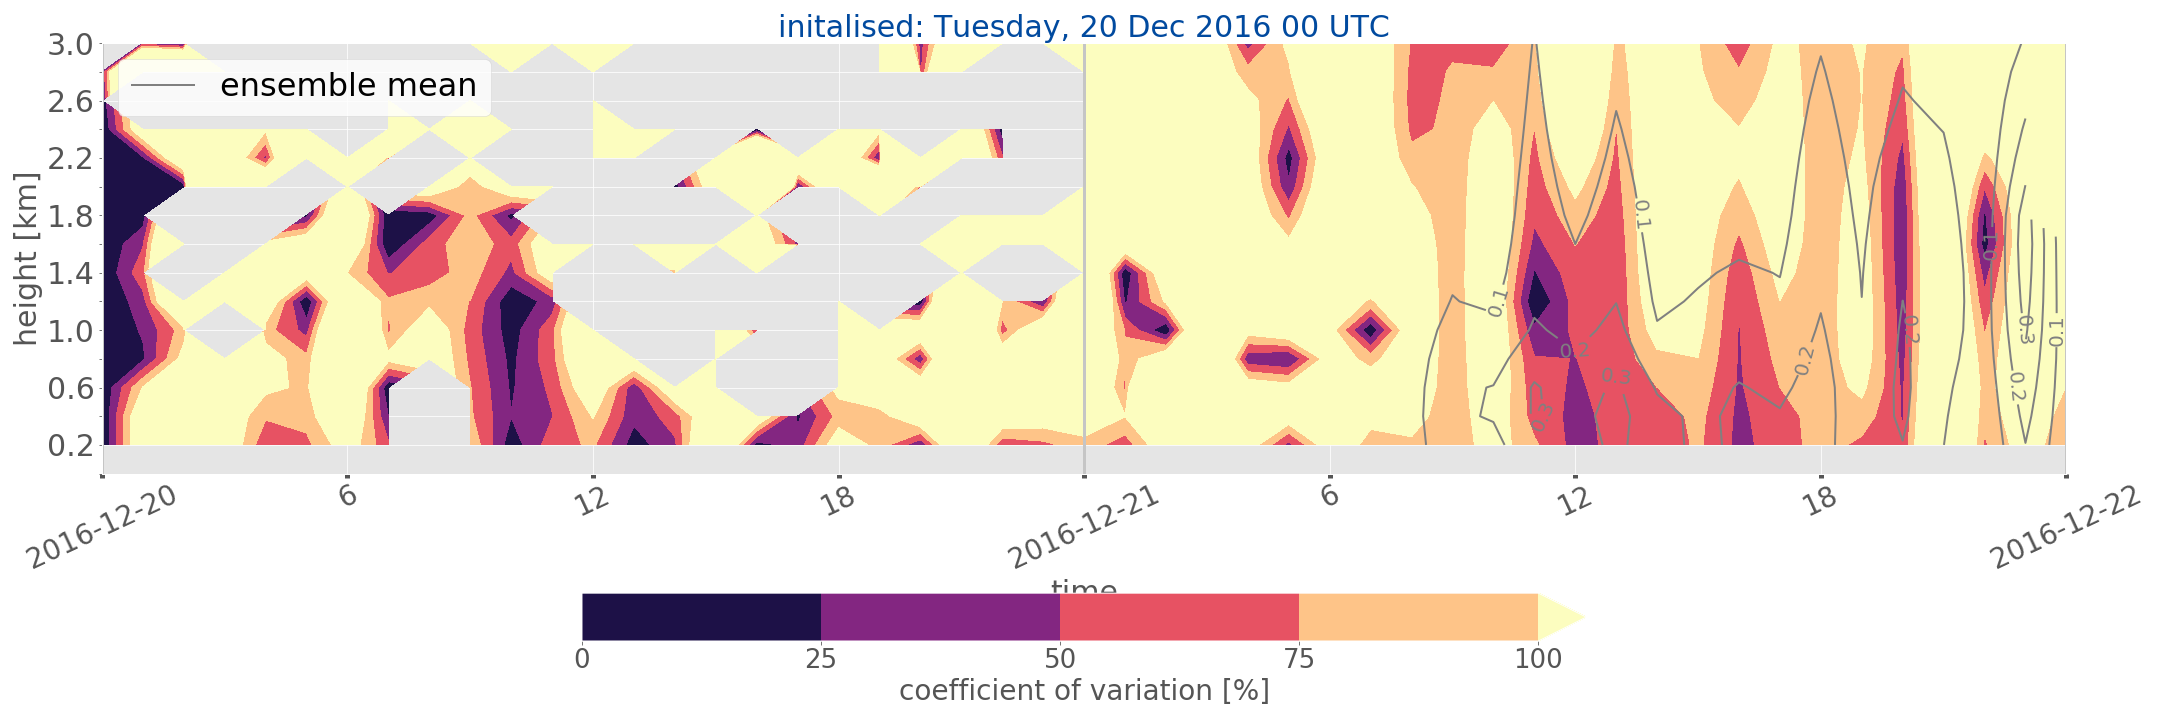
\includegraphics[trim={0.cm 5.3cm 0cm 0cm},clip,width=\textwidth]{./fig_variation/20161220}
			\caption{}\label{fig:ens_vari20}
		\end{subfigure}
%\end{figure}
%\begin{figure}\ContinuedFloat
    % 21/12
		\begin{subfigure}[t]{\textwidth}		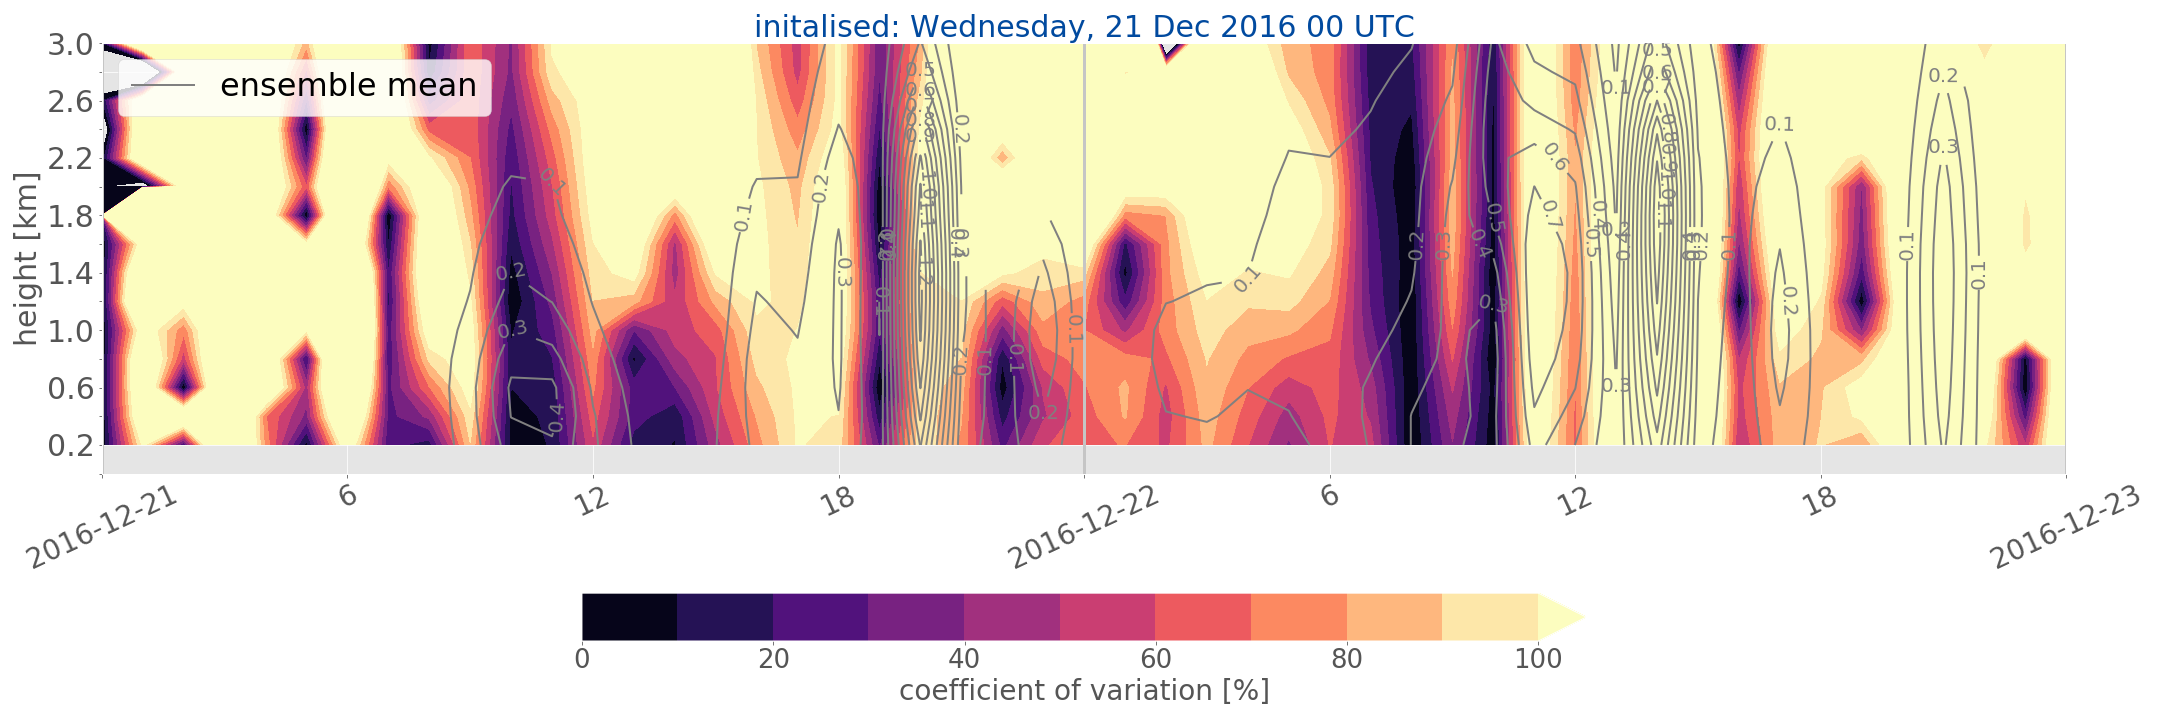
\includegraphics[trim={0.cm 5.3cm 0cm 0cm},clip,width=\textwidth]{./fig_variation/20161221}
			\caption{}\label{fig:ens_vari21}
		\end{subfigure}
       
       % colourbar
     	\begin{subfigure}[t]{\textwidth}		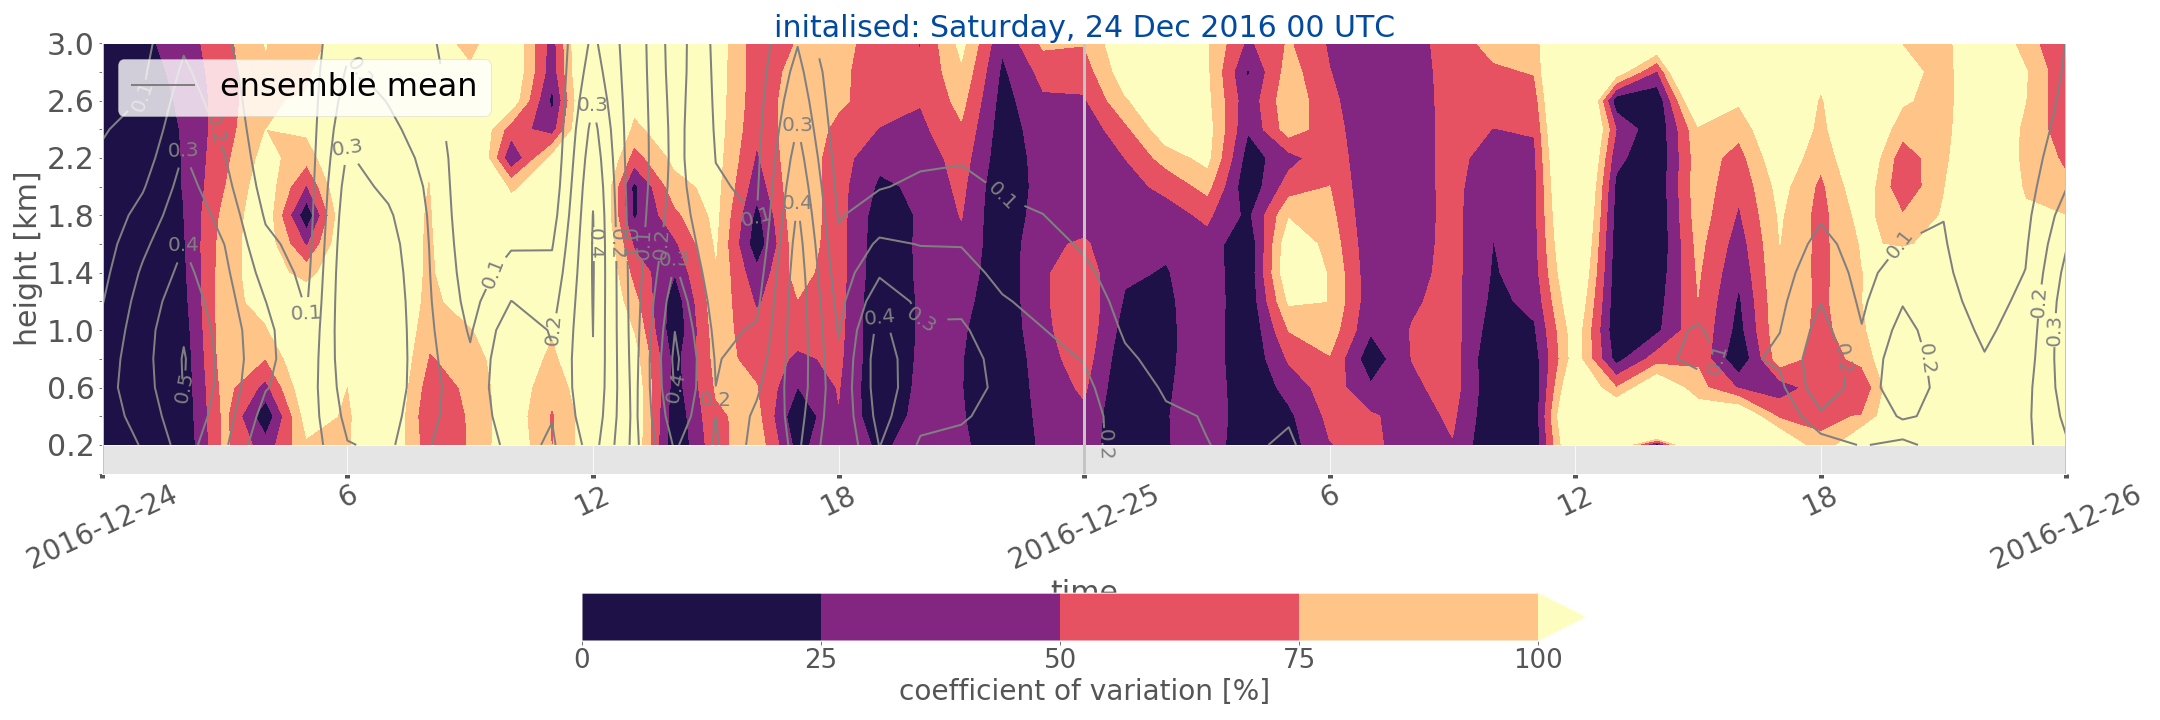
\includegraphics[trim={15.cm 0cm 15cm 21cm},clip,width=\textwidth]{./fig_variation/20161224}
		\end{subfigure}
\end{figure}
\begin{figure}[t]\ContinuedFloat
    % 22/12
		\begin{subfigure}[t]{\textwidth}		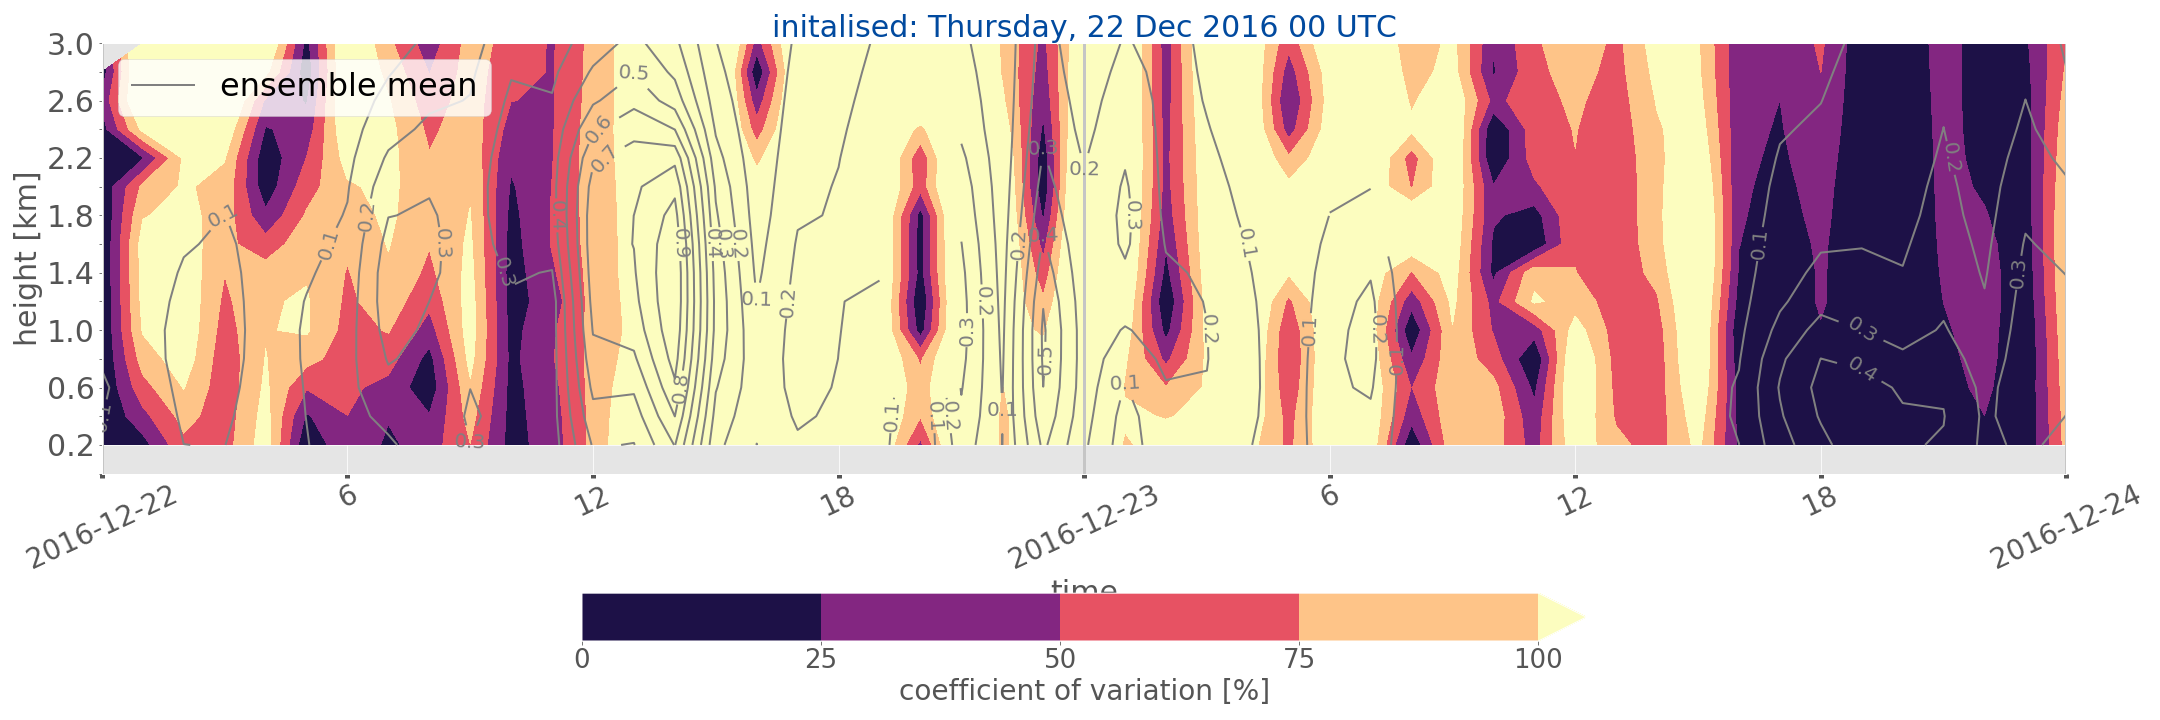
\includegraphics[trim={0.cm 5.3cm 0cm 0cm},clip,width=\textwidth]{./fig_variation/20161222}
			\caption{}\label{fig:ens_vari22}
		\end{subfigure}
    % 23/12
% 		\begin{subfigure}[t]{\textwidth}		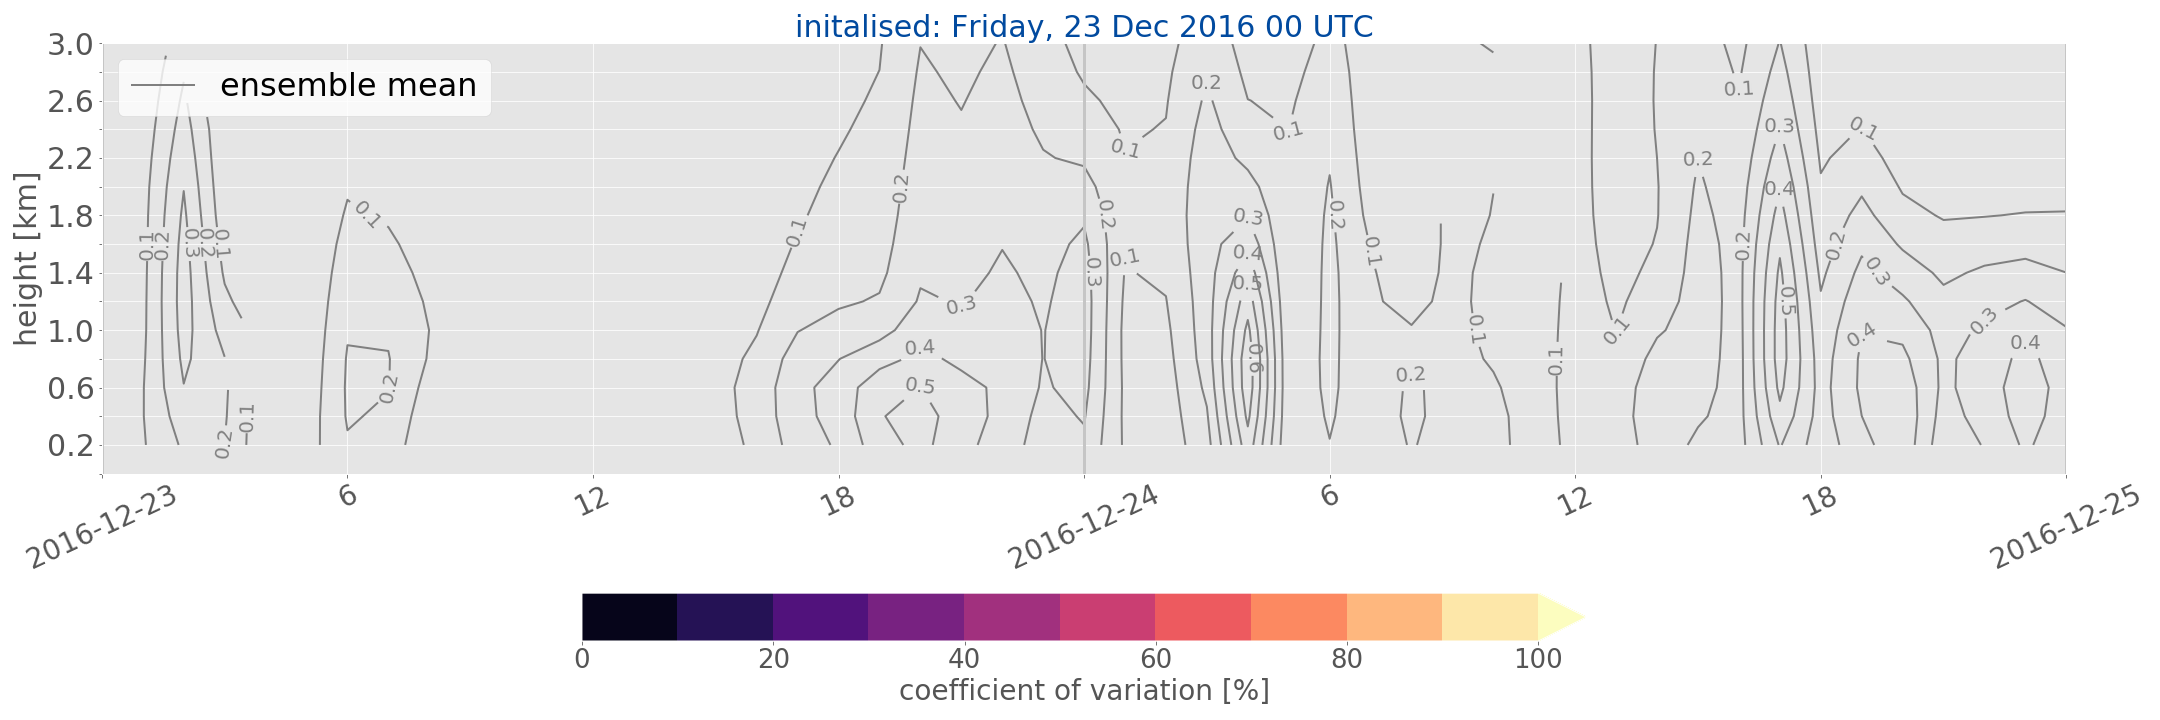
\includegraphics[trim={0.cm 0cm 0cm 0cm},clip,width=\textwidth]{./fig_variation/20161223}
% 			\caption{}\label{fig:ens_vari23}
% 		\end{subfigure}
    % 24/12
		\begin{subfigure}[t]{\textwidth}		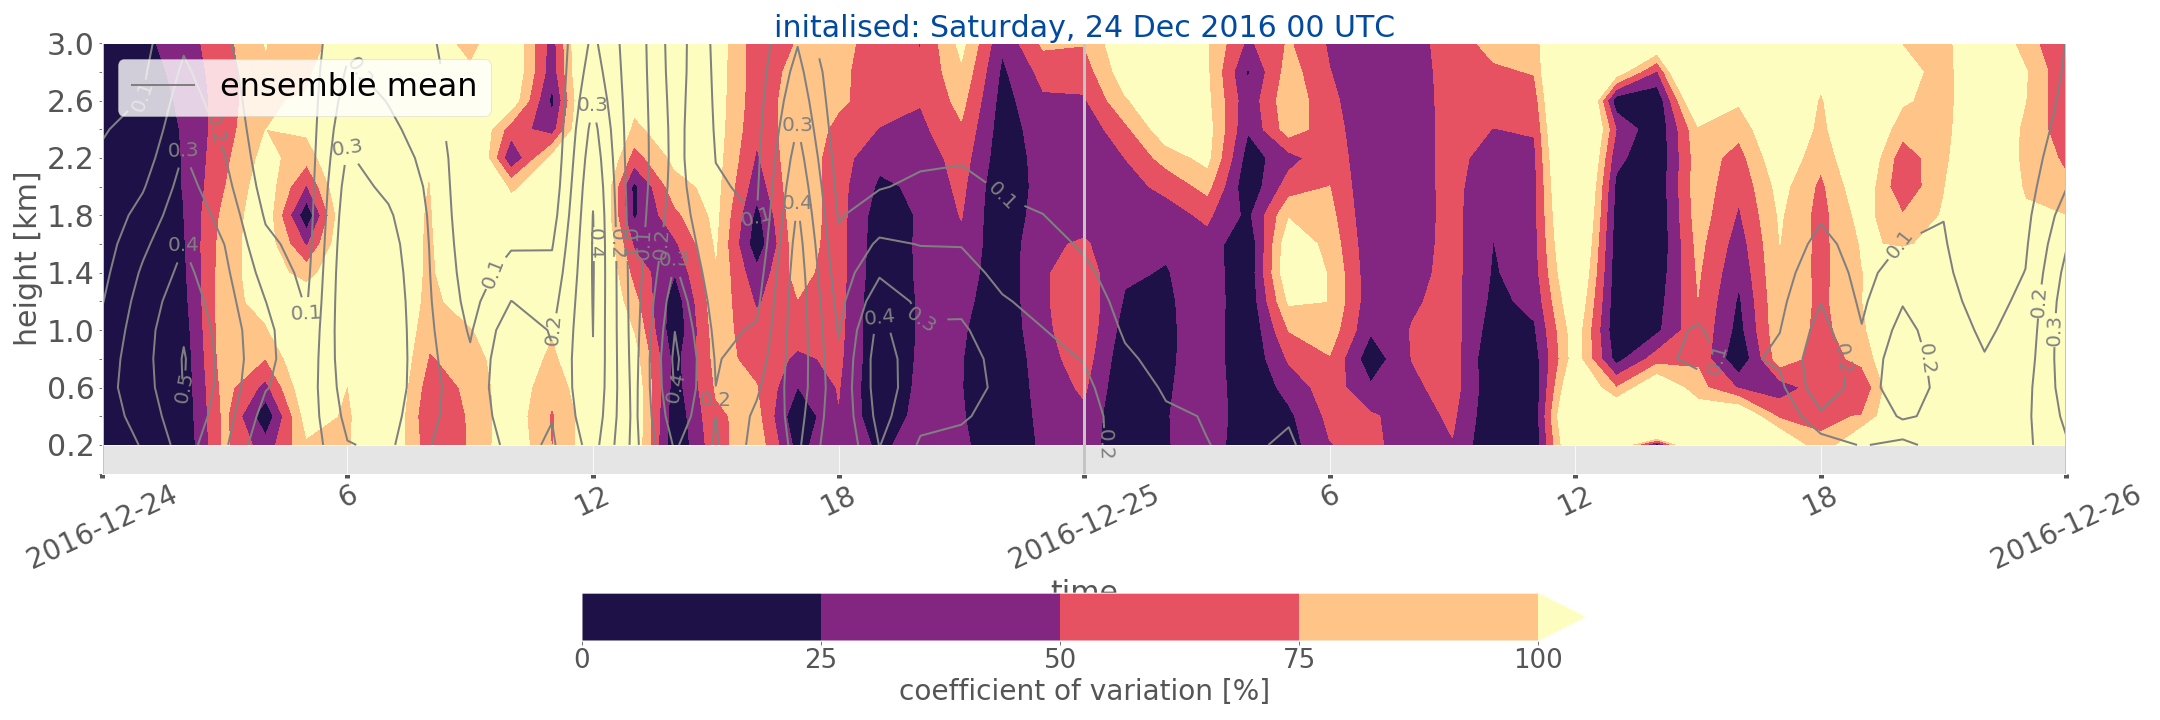
\includegraphics[trim={0.cm 5.3cm 0cm 0cm},clip,width=\textwidth]{./fig_variation/20161224}
			\caption{}\label{fig:ens_vari24}
		\end{subfigure}
        
     % colourbar
     	\begin{subfigure}[t]{\textwidth}		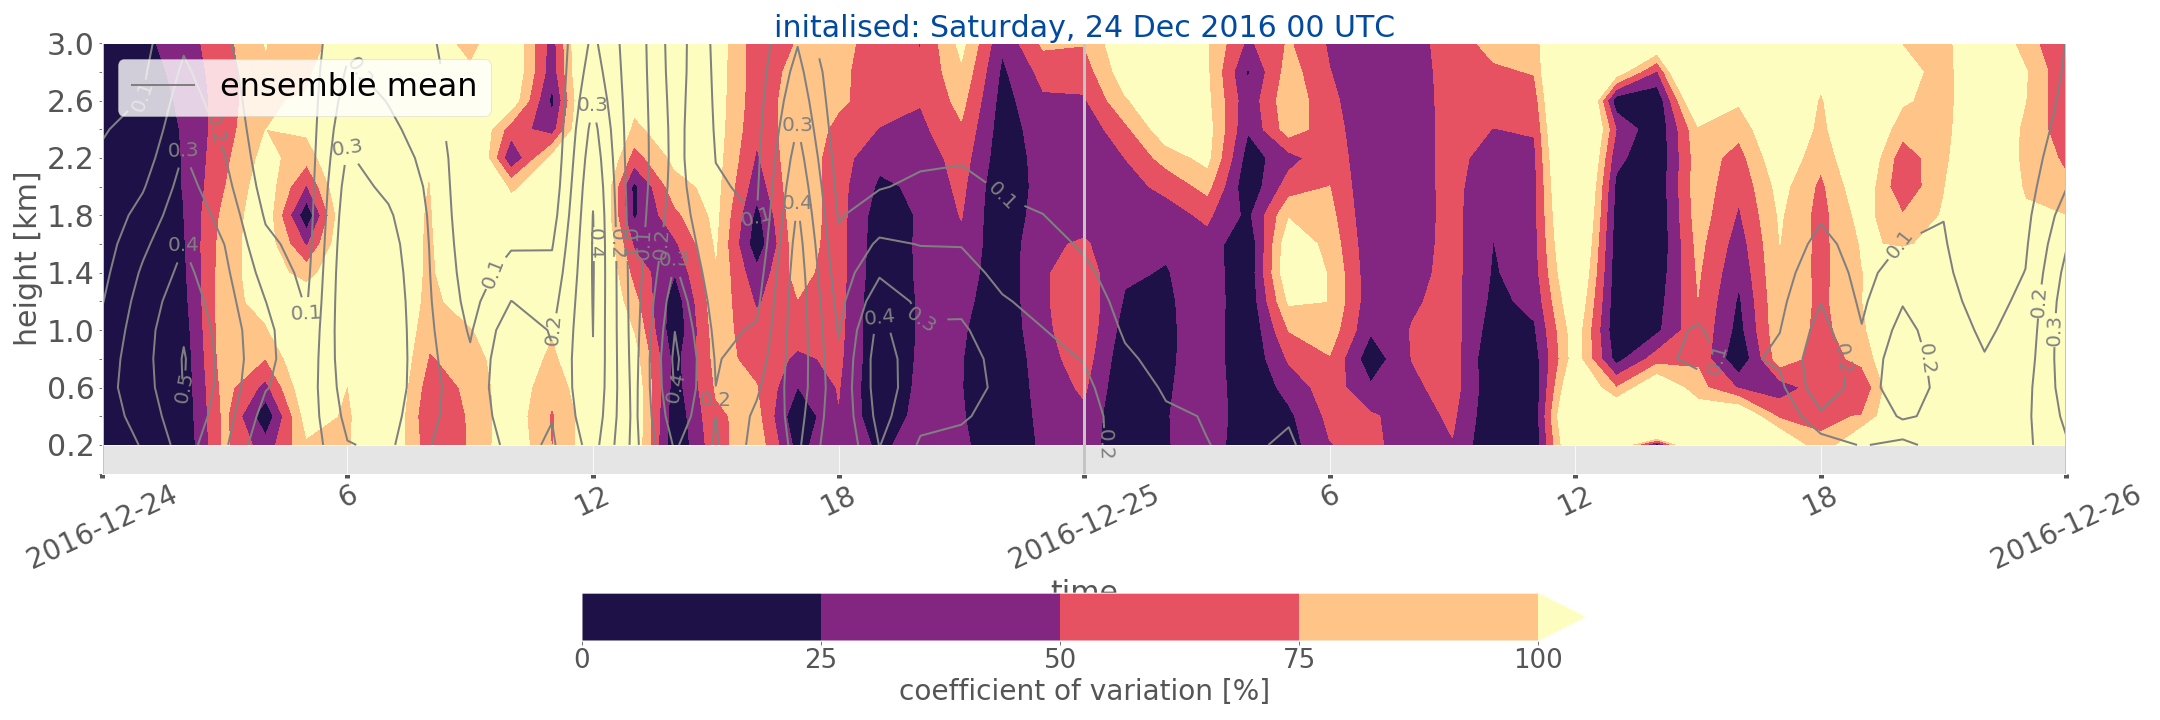
\includegraphics[trim={15.cm 0cm 15cm 21cm},clip,width=\textwidth]{./fig_variation/20161224}
		\end{subfigure}
\end{figure}
\begin{figure}[t]\ContinuedFloat
	\centering
    % 25/12
		\begin{subfigure}[t]{\textwidth}		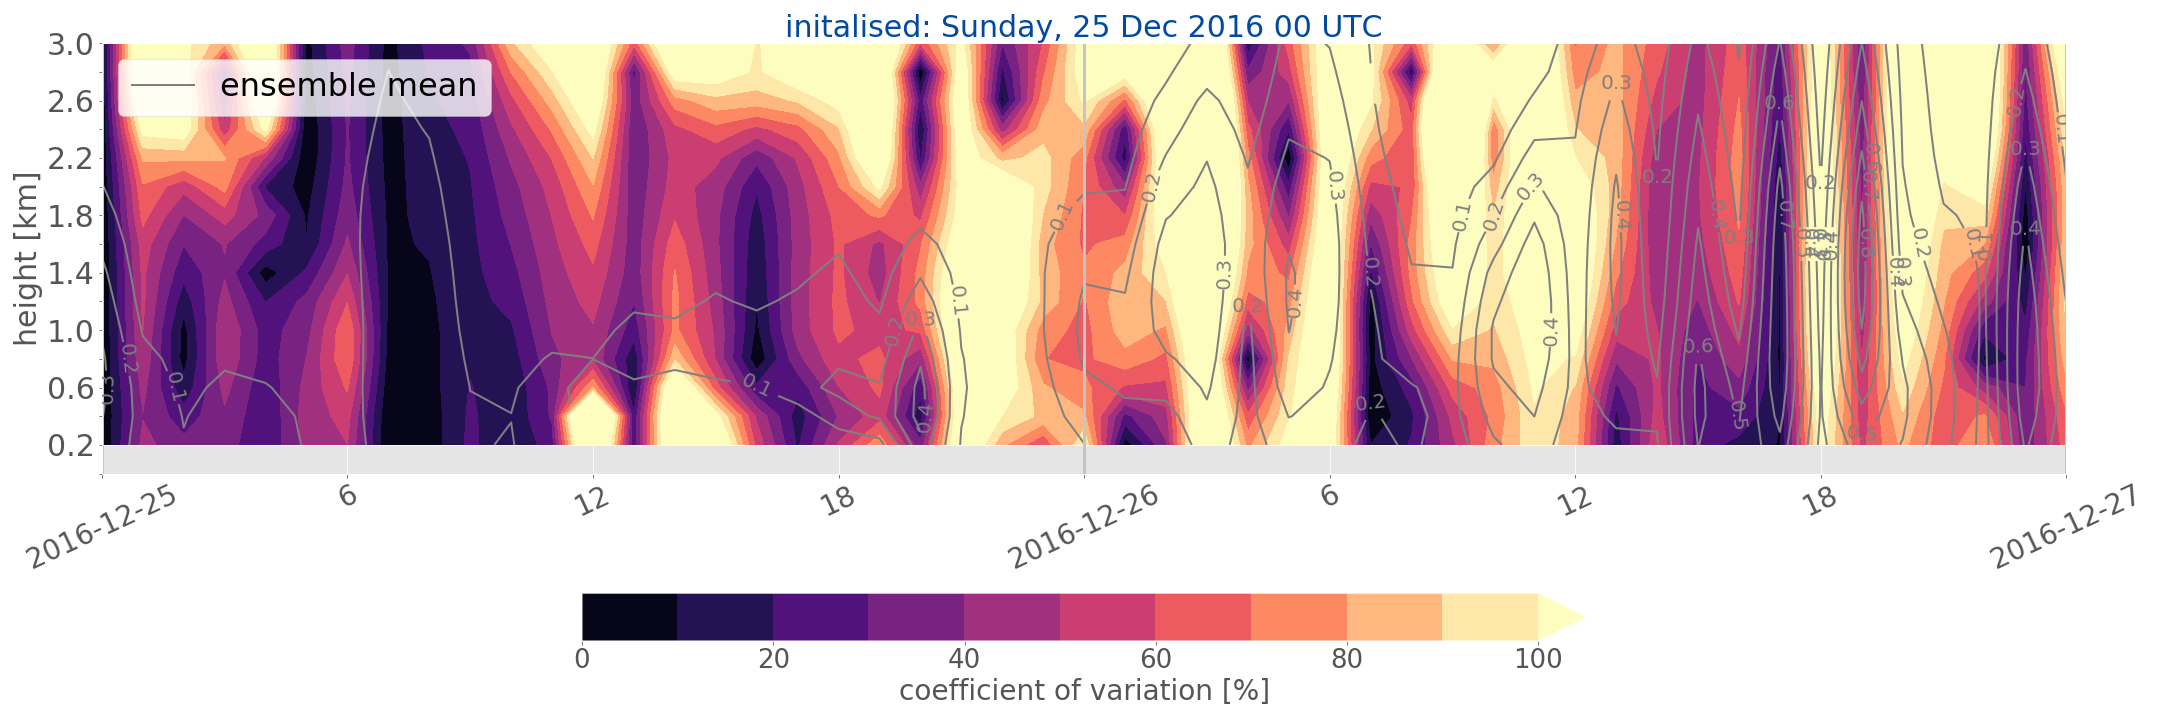
\includegraphics[trim={0.cm 5.3cm 0cm 0cm},clip,width=\textwidth]{./fig_variation/20161225}
			\caption{}\label{fig:ens_vari25}
		\end{subfigure}
    % 26/12
		\begin{subfigure}[t]{\textwidth}		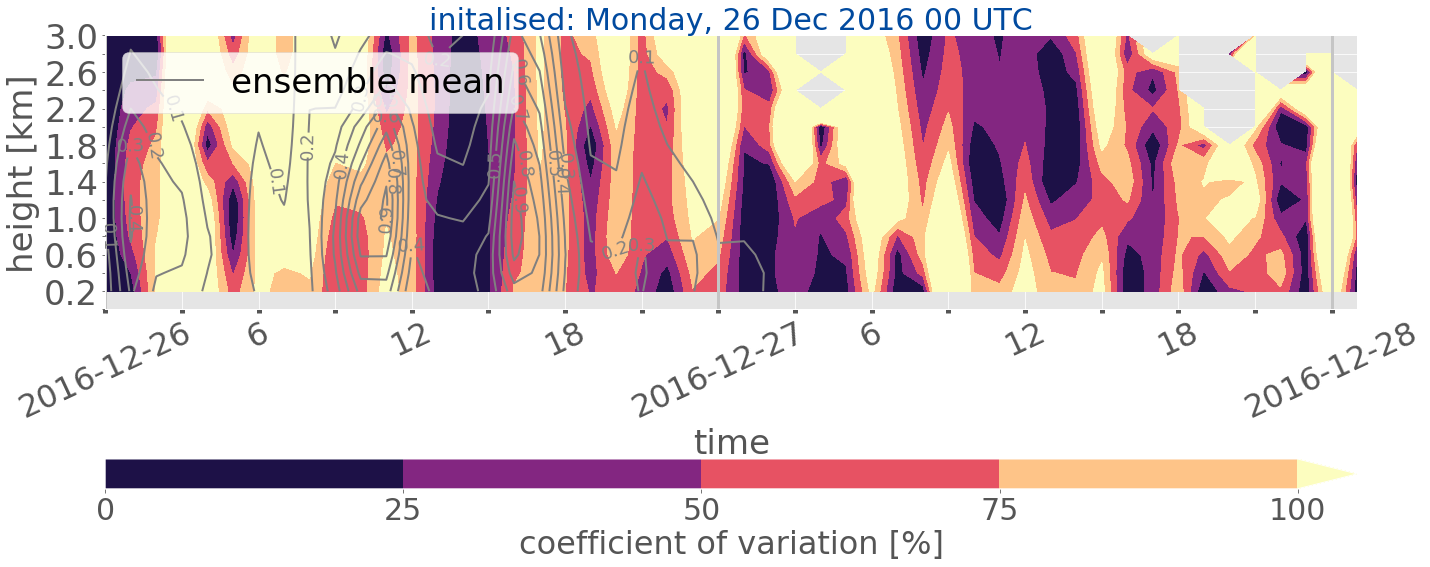
\includegraphics[trim={0.cm 5.3cm 0cm 0cm},clip,width=\textwidth]{./fig_variation/20161226}
			\caption{}\label{fig:ens_vari26}
		\end{subfigure}
%     % 27/12
% 		\begin{subfigure}[t]{\textwidth}		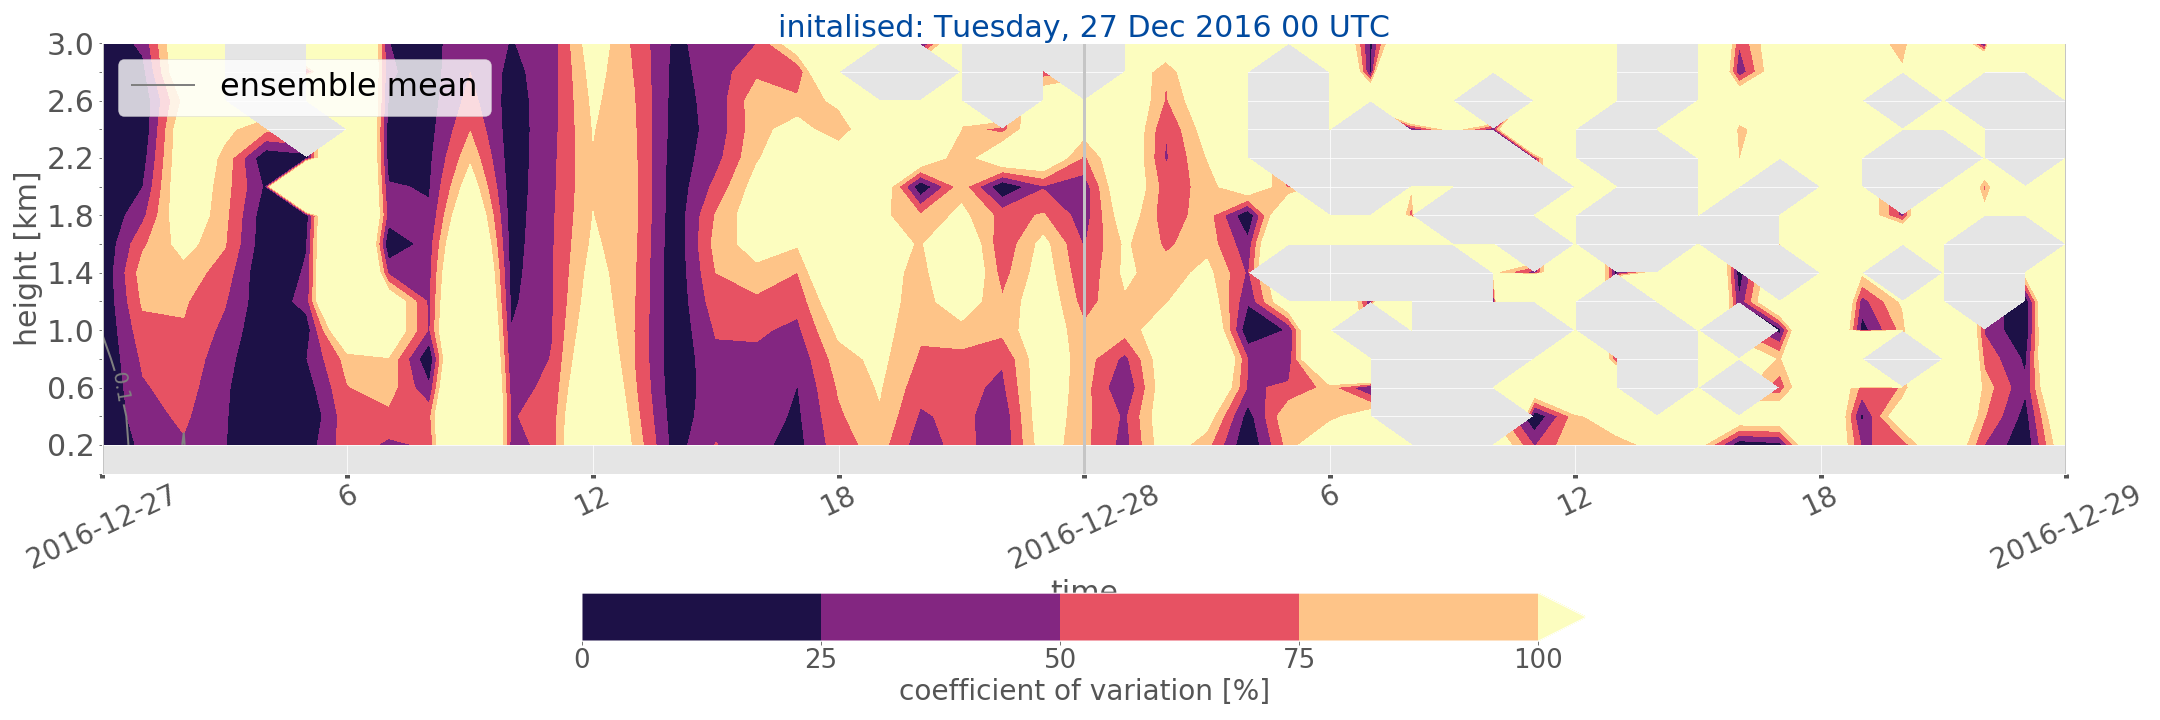
\includegraphics[trim={0.cm 5.3cm 0cm 0cm},clip,width=\textwidth]{./fig_variation/20161227}
% 			\caption{}\label{fig:ens_spread27}
% 		\end{subfigure}
        
    % colourbar
     	\begin{subfigure}[t]{\textwidth}		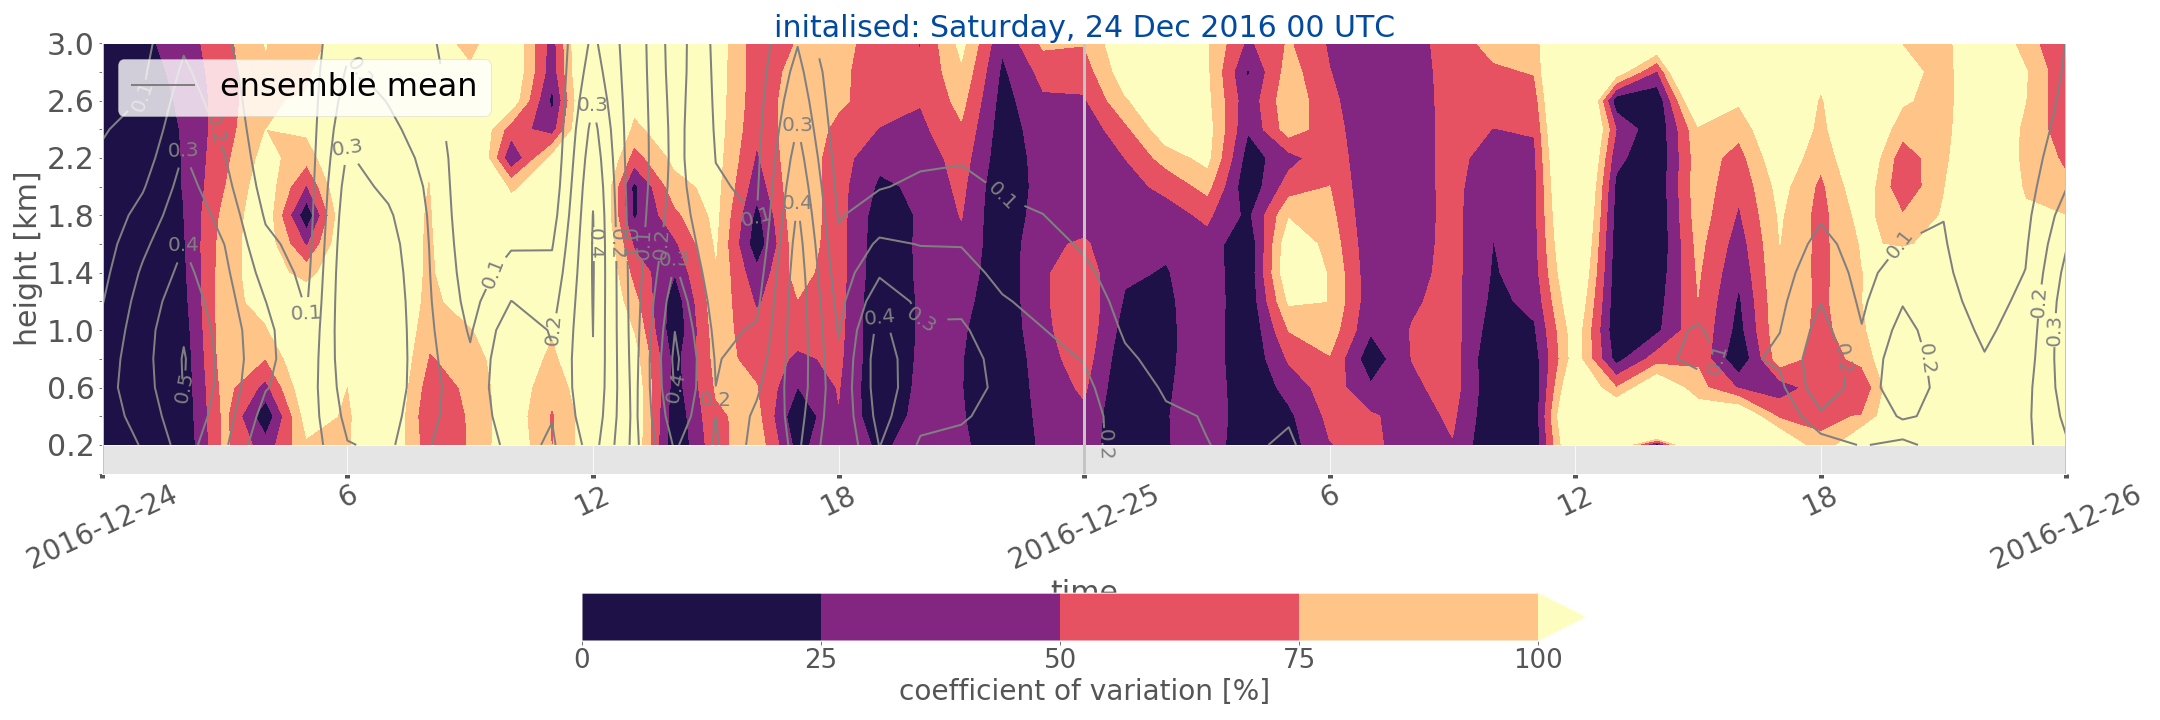
\includegraphics[trim={15.cm 0cm 15cm 21cm},clip,width=\textwidth]{./fig_variation/20161224}
		\end{subfigure}
        \caption{SWC variation of the ten ensemble members of MEPS. The lighter the colour according to the colourbar the higher the variation between the perturbed ensemble members. In grey the ensemble mean of all ten members.}\label{fig:ens_vari}
\end{figure}


%%%%%%%%%%%%%%%%%%%%%%%%%%%%%%%%%%%%%%%%%%%%%%%%%%%%%%%%%%%%%%%%%%%%%%%%%%
To verify how well the ensemble forecast system MEPS has performed, a verification is performed as described in \Cref{sec:ens_mean_spread}. \Cref{fig:ens_vari20,fig:ens_vari21,fig:ens_vari22,fig:ens_vari24,fig:ens_vari25,fig:ens_vari26} show the coefficient of variation for SWC, which is the standard deviation of the ten ensemble members divided by the mean of all ensemble members. This coefficient gives the possibility to compare the SWC results for different days with different values. It also shows if the ensemble spread (standard deviation of all ensemble members) is low the SWC is does not need to be less variable.
\\
The grey line in \Cref{fig:ens_vari} shows the ensemble mean as a contour. The darker the colour in \Cref{fig:ens_vari} the smaller is the variation of SWC relative to the mean. The \SI{23}{\dec} does not exist, because it had too few ensemble members (only six) to create a reasonable verification and therefore is the ensemble mean in \Cref{fig:SWC23} classified as very uncertain. The interpretation of the coefficient of variation for SWC is presented in \Cref{tab:verification}.
% %%% table verification %%%%%%%%%%%%%%%%%%%%%%%%%%%%%%%%%%%%%
\begin{table}[t!]
	\begin{center}
		\caption{Interpretation of the coefficient of variation for SWC.} \label{tab:verification}
		\begin{tabular}{c|c|c}
			\hline\hline
			\textbf{Size of CV} & \multicolumn{2}{c}{\textbf{Interpretation}} \\ 
			\SI{}{\percent} & variability & forecast accuracy \\ \hline \hline 
			\numrange{0}{< 25} & negligible & very high  \\ \hline
			\numrange{25}{< 50} & low & high \\ \hline
			\numrange{50}{< 75} & moderate & moderate \\ \hline
			\numrange{75}{< 100} & high & low \\ \hline
			\num{100} to $\infty$ & very high & no  \\ \hline \hline
		\end{tabular}
	\end{center}
\end{table}
%%%%%%%%%%%%%%%%%%%%%%%%%%%%%%%%%%%%%%%%%%%%%%%%%%%%%%%%%%%%%%%%%%%%%%%%%%
%
A small CV indicates a very high forecast accuracy, since the variability is negligible between the ten ensemble members (\SIrange{0}{< 25}{\percent}). Similar is a large CV associated with a low forecast accuracy and therefore a very high variability between the members (\SI{> 100}{\percent}). As expected increases the forecast uncertainty with increasing prediction time. It is still possible that in some cases the CV will be larger with a shorter prediction time than with a longer lead time. This could be the case, when strong synoptic systems with complex structure are apparent.
\\
In some cases increases the forecast accuracy with lead time. It also shows, that the CV agrees well with the prediction of the up-slope events and is more often uncertain about the pulsing part, when west wind is observed. 
\\
\\
The \SI{21}{\dec} contained an up-slope event between \SIrange{9}{13}{\UTC} and a wind change to west followed a pulsed precipitation afterwards. The coefficient of variation of the SWC in \Cref{fig:ens_vari20} shows a variation of up to \SI{100}{\percent} for the up-slope and more than \SI{100}{\percent} for the pulsed part, when initialised on \SI{20}{\dec}. An initialisation on \SI{21}{\dec} gives a better result, were the variation is less with a pronounced accuracy of up to \SI{30}{\percent} for the up-slope part around noon. 
The variation shows another good agreement around \SI{19}{\UTC}, one hour prior the maximum predicted mean SWC. For the maximum observed SWC is the CV higher than \SI{90}{\percent} and thus no forecast accuracy exists. This maximum followed from the fact, that the deterministic forecast is the strongest at time and all other ensemble members respond with a weaker SWC. The very high variability and the discrepancy between the ensemble members will be discussed further in \Cref{sec:vertEM09:2112}.
\\
While the ensemble mean produced a high SWC at \SIlist{11;14}{\UTC} on the \SI{22}{\dec}, shows the variation of SWC a very high variability at this times, when initialised on \SI{21}{\dec} (\Cref{fig:ens_vari21}). This follows a high uncertainty of the SWC peak values in \Cref{fig:SWC21}, whereas it is very certain some hours before when almost no snow water content was present. 
For an initialisation on \SI{22}{\dec} is the peak around \SI{11}{\UTC} merged together with the one at \SI{14}{\UTC}. The CV in \Cref{fig:ens_vari22} displays again a very high forecast accuracy (\SI{< 25}{\percent}) for little SWC and very high variability when the SWC peaks were observed. A moderate to low forecast accuracy can be seen around \SI{3}{\UTC} when the SWC is not higher than \SI{0.3}{\SWC}. 
A reason for this discrepancy is again due to the very high predicted SWC performed by the first ensemble member (\Cref{fig:EM09_22}). Here it shows, that six ensemble members would predict a high SWC around noon, which almost agrees with the vertical retrieved SWC. The pulsing after \SI{18}{\UTC} is forecasted by the first ensemble member and the forth, fifth, and seventh show a possibility of precipitation as well. 
According to the CV in \Cref{fig:ens_vari21} and \ref{fig:ens_vari22} exists there no forecast accuracy for the predicted peaks and the forecasts are only reliable when there is almost no SWC predicted. On \SI{22}{\dec} shows the forecast for initialisations more than \SI{24}{\hour} and less than \SI{24}{\hour} prior a pattern as for few precipitation is the forecast accuracy high to very high and for higher SWC is the forecast accuracy not existing. 
\\
All ensemble members agree well with the occurrence of the up-slope storm on \SI{23}{\dec} (\Cref{fig:EM09_22}). The verification in \Cref{fig:ens_vari22} shows little discrepancy below \SI{50}{\percent} with most having a high forecast accuracy. All ten ensemble members forecast the up-slope to occur after \SI{17}{\UTC}, compare \Cref{fig:EM09_22}. While comparing only six ensemble members in \Cref{fig:EM09_23}, one could assume that the uncertainty of all ensemble members during the up-slope storm is low, but not as certain as for an initialisation on \SI{22}{\dec} at \SI{0}{\UTC}. 
The deterministic forecast (EM0) and ensemble member one in \Cref{fig:EM09_22} indicate peaks of high SWC before \SI{7}{\UTC}. The retrieved SWC on \SI{23}{\dec} had two peaks, one at around \SI{2}{\UTC} and another at \SI{5}{\UTC}. The first ensemble member predicted the peak just to occur in between and a second at \SI{7}{\UTC}. Overall seems the first ensemble member of the  \SI{22}{\dec} initialisation to be a good forecast when comparing to the retrieved SWC in \Cref{fig:SWC22}.
\\
The \SI{24}{\dec} was one of the days, where pulsing of the storm was observed and predicted throughout the day. 
\Cref{fig:EM09_23} can give an idea about the variation between the six existing forecasts. Three ensemble members (EM0, EM7, EM8) seem to agree on the occurrence of a SWC peak around \SI{18}{\UTC}, which would be in the range of a moderate forecast accuracy. 
For an initialisation on \SI{24}{\dec} indicates the variation coefficient of all ten ensemble members in \Cref{fig:ens_vari24} different accuracies. The ensemble mean is presented in grey and shows the pulses forecasted. Until noon on \SI{24}{\dec} is no forecast accuracy for the peaks. The peak observed at \SI{14}{\UTC} indicates a low variability between the ensemble members. The peak at \SI{17}{\UTC} has a high accuracy up to \SI{0.8}{\km} and moderate up to \SI{1.2}{\km}. After \SI{19}{\hour} forecast time is the variability between the ensemble members negligible and all agree on the existence of precipitation.
A detail inter-comparison between the surface accumulation and the vertical snow water content is presented in \Cref{sec:vertEM09:2412}.
\\
In general was the \SI{25}{\dec} a very weak snow storm with strong liquid precipitation observed between \SIlist{12;18}{\UTC}. \Cref{fig:SWC24} and \Cref{fig:SWC25} gave a low value of predicted SWC in the course of a day. As \Cref{fig:ens_vari24} indicates is the forecast accuracy very high up to \SI{1.8}{\km} until noon, this is when liquid precipitation was measured. According to \Cref{fig:LWC24} and \ref{fig:LWC25} was the depth of the liquid layer up to \SI{0.8}{\km}. The variation coefficient has a large disagreement below \SI{0.8}{\km}, but above is the variability between the members not existing or low. The weak peak in \Cref{fig:SWC25} at \SI{18}{\UTC} had a moderate forecast accuracy, were it is afterwards very high. For an initialisation on \SI{25}{\dec} is the forecast accuracy high until noon (\Cref{fig:ens_vari25}). While liquid precipitation was monitored is the accuracy in the lower layer first not existing and shortly before \SI{18}{\UTC} very high. A high agreement exists for the SWC peak up to \SI{0.8}{\km} and decreases to be moderate above. A discussion about the precipitation change and its related forecast is given in \Cref{sec:vertEM09:2512}.
\\
Again, the \SI{26}{\dec} is only comparable until \SI{17}{\UTC} even though \Cref{fig:SWC25} would suggest a continues pulsing of the storm. The two peaks around \SI{18}{\UTC} (\Cref{fig:SWC25}) are forecasted with a very high and moderate accuracy in \Cref{fig:ens_vari25}. The SWC peaks at around \SIlist{2;5}{\UTC} show a very high variability. \Cref{fig:EM09_25} shows that four out of ten ensemble members would agree with the peaked event around \SI{5}{\UTC}. Whereas the peak at \SI{2}{\UTC} is dominated by the strong predicted SWC of the deterministic forecast, which follows the high variation in \Cref{fig:ens_vari25}. 
Initialised on \SI{26}{\dec} follows that the SWC peak at \SI{2}{\UTC} is related to a moderate forecast accuracy. Low forecast accuracy is shown for the SWC at \SI{11}{\UTC} and the one at \SI{16}{\UTC} has a low to moderate variability between the members.  When looking at \Cref{fig:EM09_26} might this disagreement be related to the colourful variation of the vertical predicted SWC. There seems no agreement between the different members about the incidence of the SWC peaks. The high conflict for the CV before noon is most likely related to the high SWC of the deterministic SWC. 
%
% \\ \\
% Another way to verify an ensemble prediction system is to use the ensemble spread of the SWC, which is just the standard deviation of all ten ensemble members, shown in \Cref{fig:ens_spread}. Here, lighter colours of the SWC show more deviation of the SWC around the ensemble mean and darker colours indicate that the ensemble members are close to the mean. Grey contour lines indicate the ensemble mean of the SWC to see any variations.
% \\
% As the results in \Cref{fig:ens_spread} show is the spread very low for the up-slope cases (\Cref{fig:ens_spread20,fig:ens_spread21,fig:ens_spread22,fig:ens_spread23}). This means that all ensemble members perform well when the wind is from the east. 
% \\
% The ensemble spread shows more uncertainty for the pulsing events. 
% Initialisation on \SIlist{21;22;26}{\UTC} shows more spread between the different ensemble members (lighter colour in \Cref{fig:ens_spread21}, \ref{fig:ens_spread22}, and \ref{fig:ens_spread26}), especially for the ensemble mean maximum values. On these days the maximum SWC was quite high and reached the overall ensemble mean maximum of \SI{1.24}{\SWC} on \SI{21}{\dec}.
% Fewer spread between the ensemble members is shown for the initialisation \SIlist{23;24;25}{\UTC} (\Cref{fig:ens_spread23,fig:ens_spread24,fig:ens_spread25}), when the ensemble mean never reached more than \SI{0.54}{\SWC}.

%%%%%%%%%%%%%%%%%%%%%%%%%%%%%%%%%%%%%%%%%%%%%%%%%%%%%%%%%%%%%%%%%%%%%%%%%
\subsection{Wednesday, \SI{21}{\dec}}
%%%%%%%%% vertical obs %%%%%%%%%%%%%%
%\subsection{Vertical snowfall observations}
\label{sec:vertEM09:2112}
% %%% image SWP %%%%%%%%%%%%%%%%%%%%%%%%%%%%%%%%%%%%%
\begin{figure}[h]
	\centering
	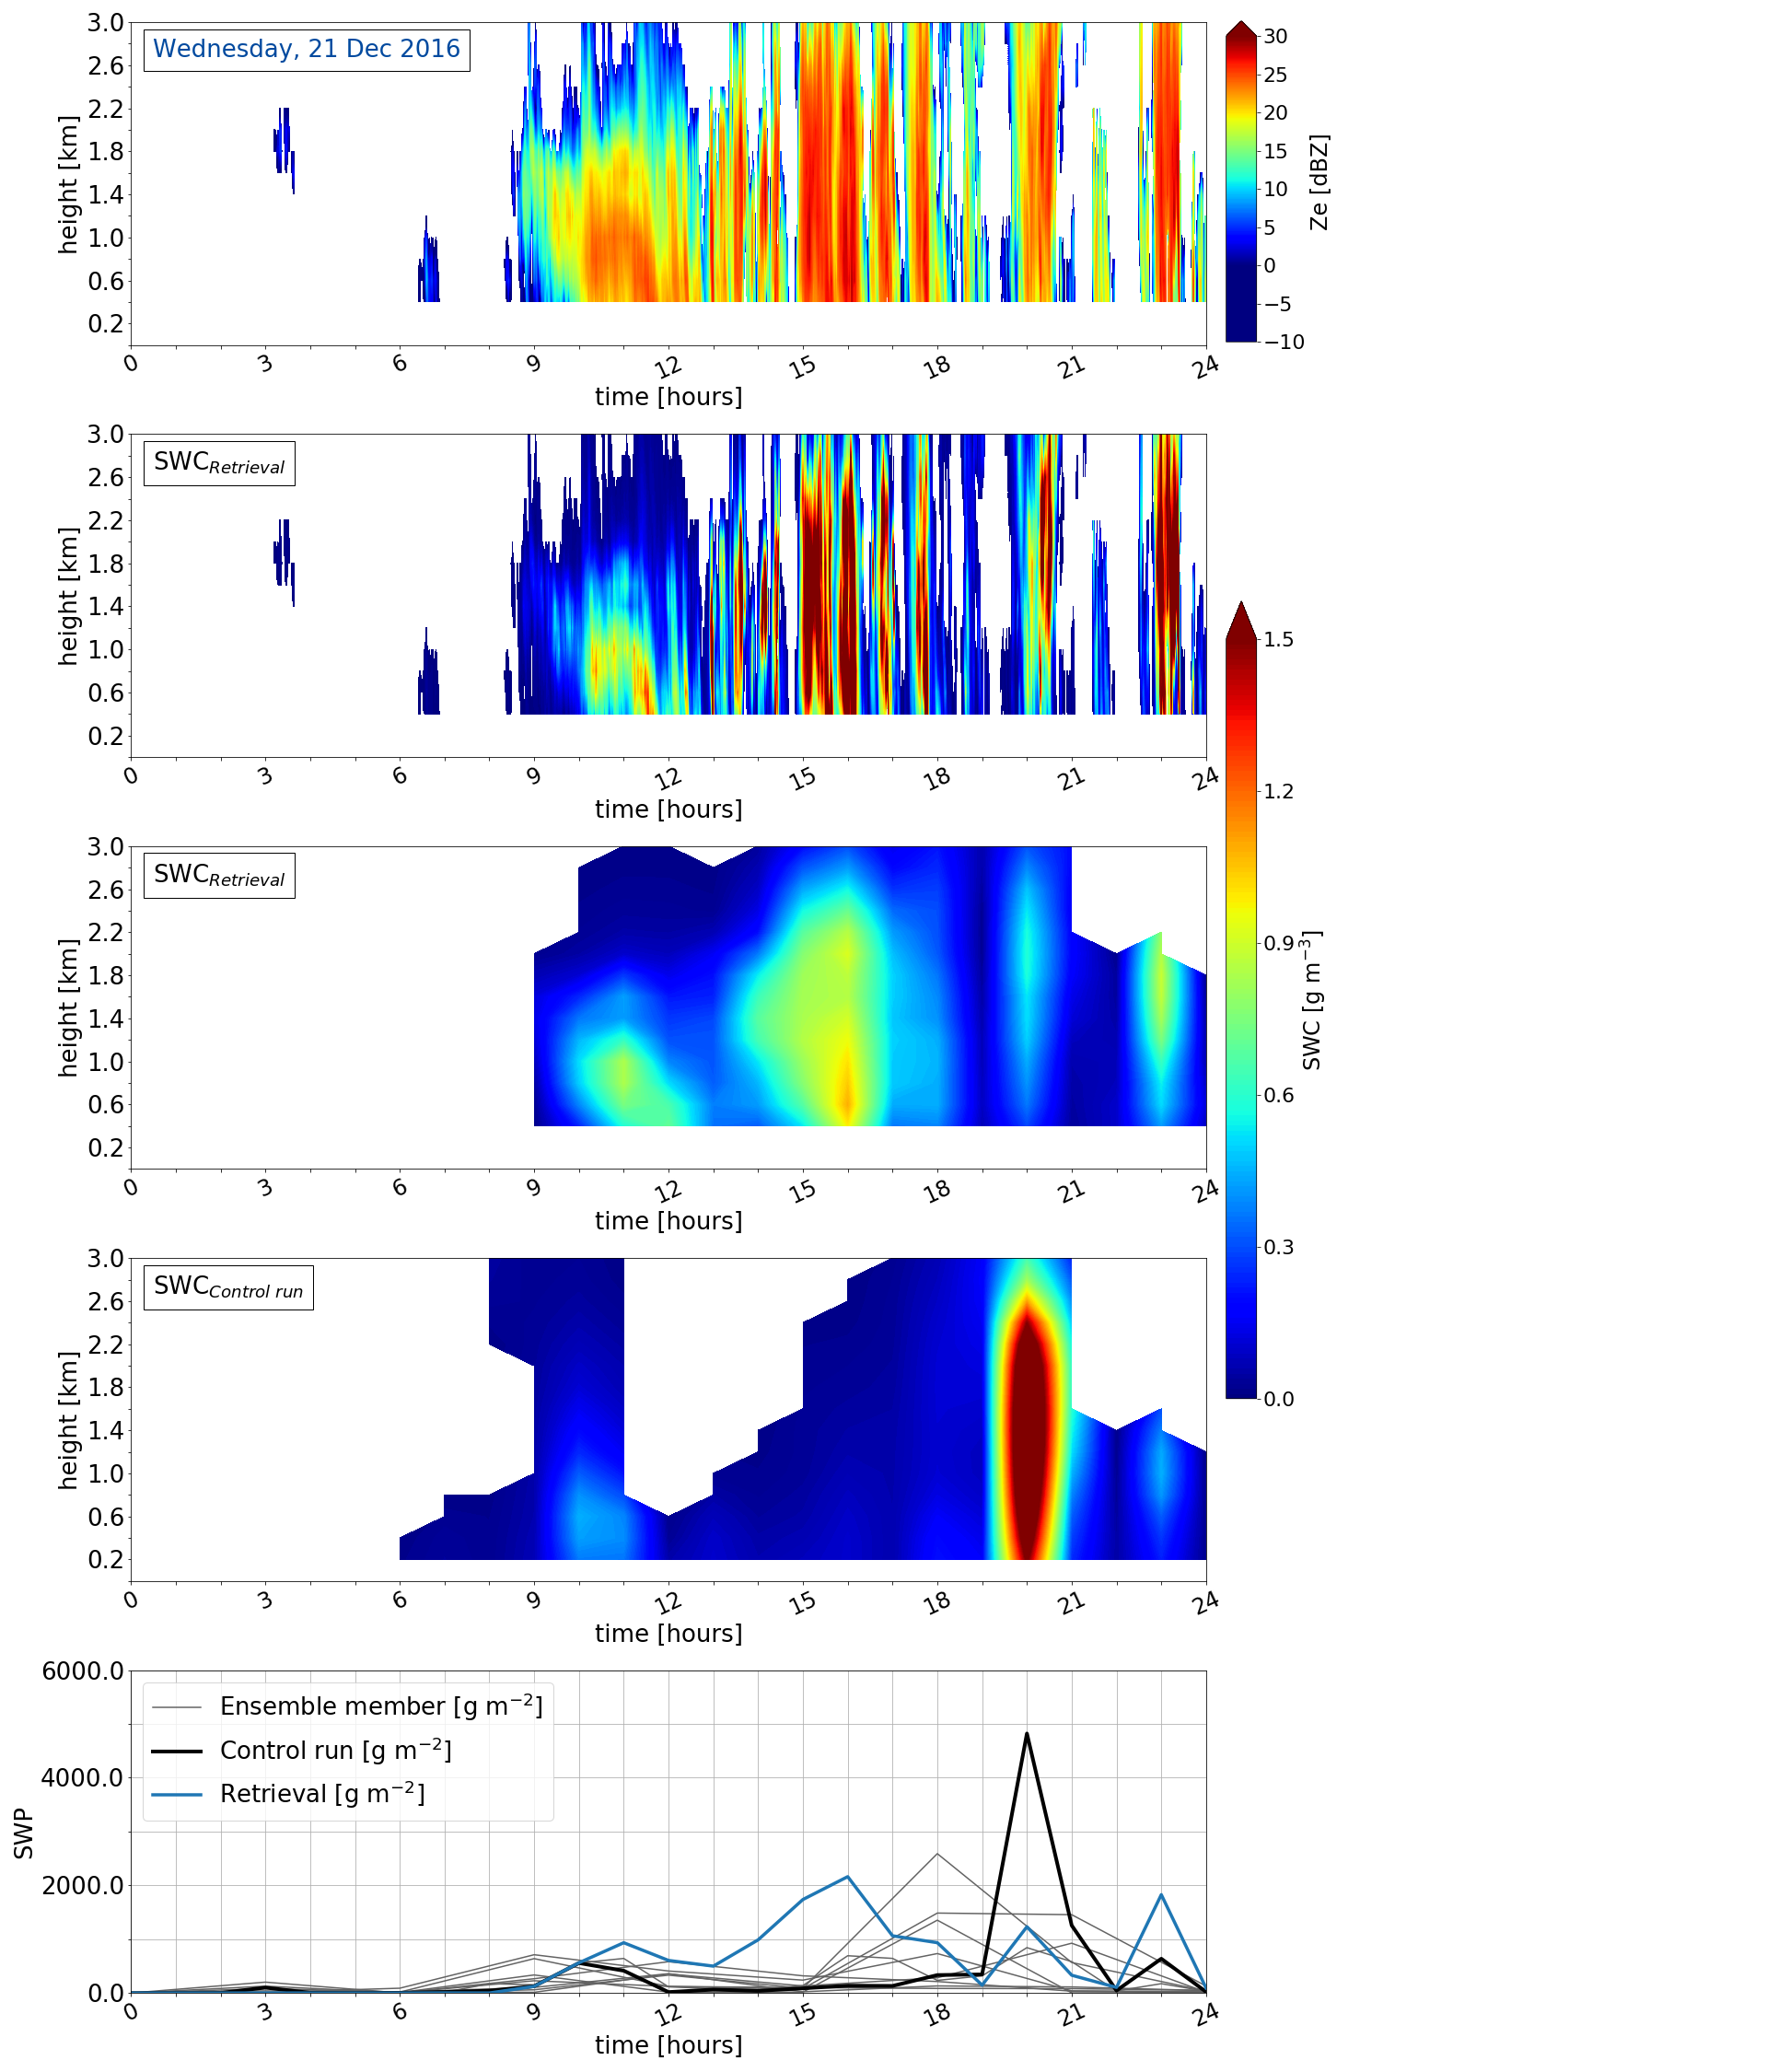
\includegraphics[trim={0.4cm .4cm 31.3cm 63.5cm},clip,width=\textwidth]{./fig_SWC/20161221}
	\caption{}\label{fig:SWP21}
\end{figure}
%%%%%%%%%%%%%%%%%%%%%%%%%%%%%%%%%%%%%%%%%%%%%%%%%%%%%%%%%%%%%%%%%%%%%%%%%%
It shows from the SWP image in \Cref{fig:SWP21}, that the deterministic forecast of MEPS (black line) dominates. Most of the other ensemble members (grey line) prognoses the daily maximum snowfall amount two hours earlier than the deterministic forecast. The blue, dashed line, indicating the ensemble mean SWP shows the weakening of the snowfall amount when taking the average of all ten ensemble members with a maximum value at \SI{20}{\UTC}. By comparing the orange line (SWP from the retrieval) and the blue, dashed line it shows, that the ensemble mean value of MEPS gets closer to the observed one, \SIlist{2833; 2162}{\SWP} respectively.
%
% %%% image ensemble member 0-9 %%%%%%%%%%%%%%%%%%%%%%%%%%%%%%%%%%%%%
\begin{figure}[t]
	\centering
	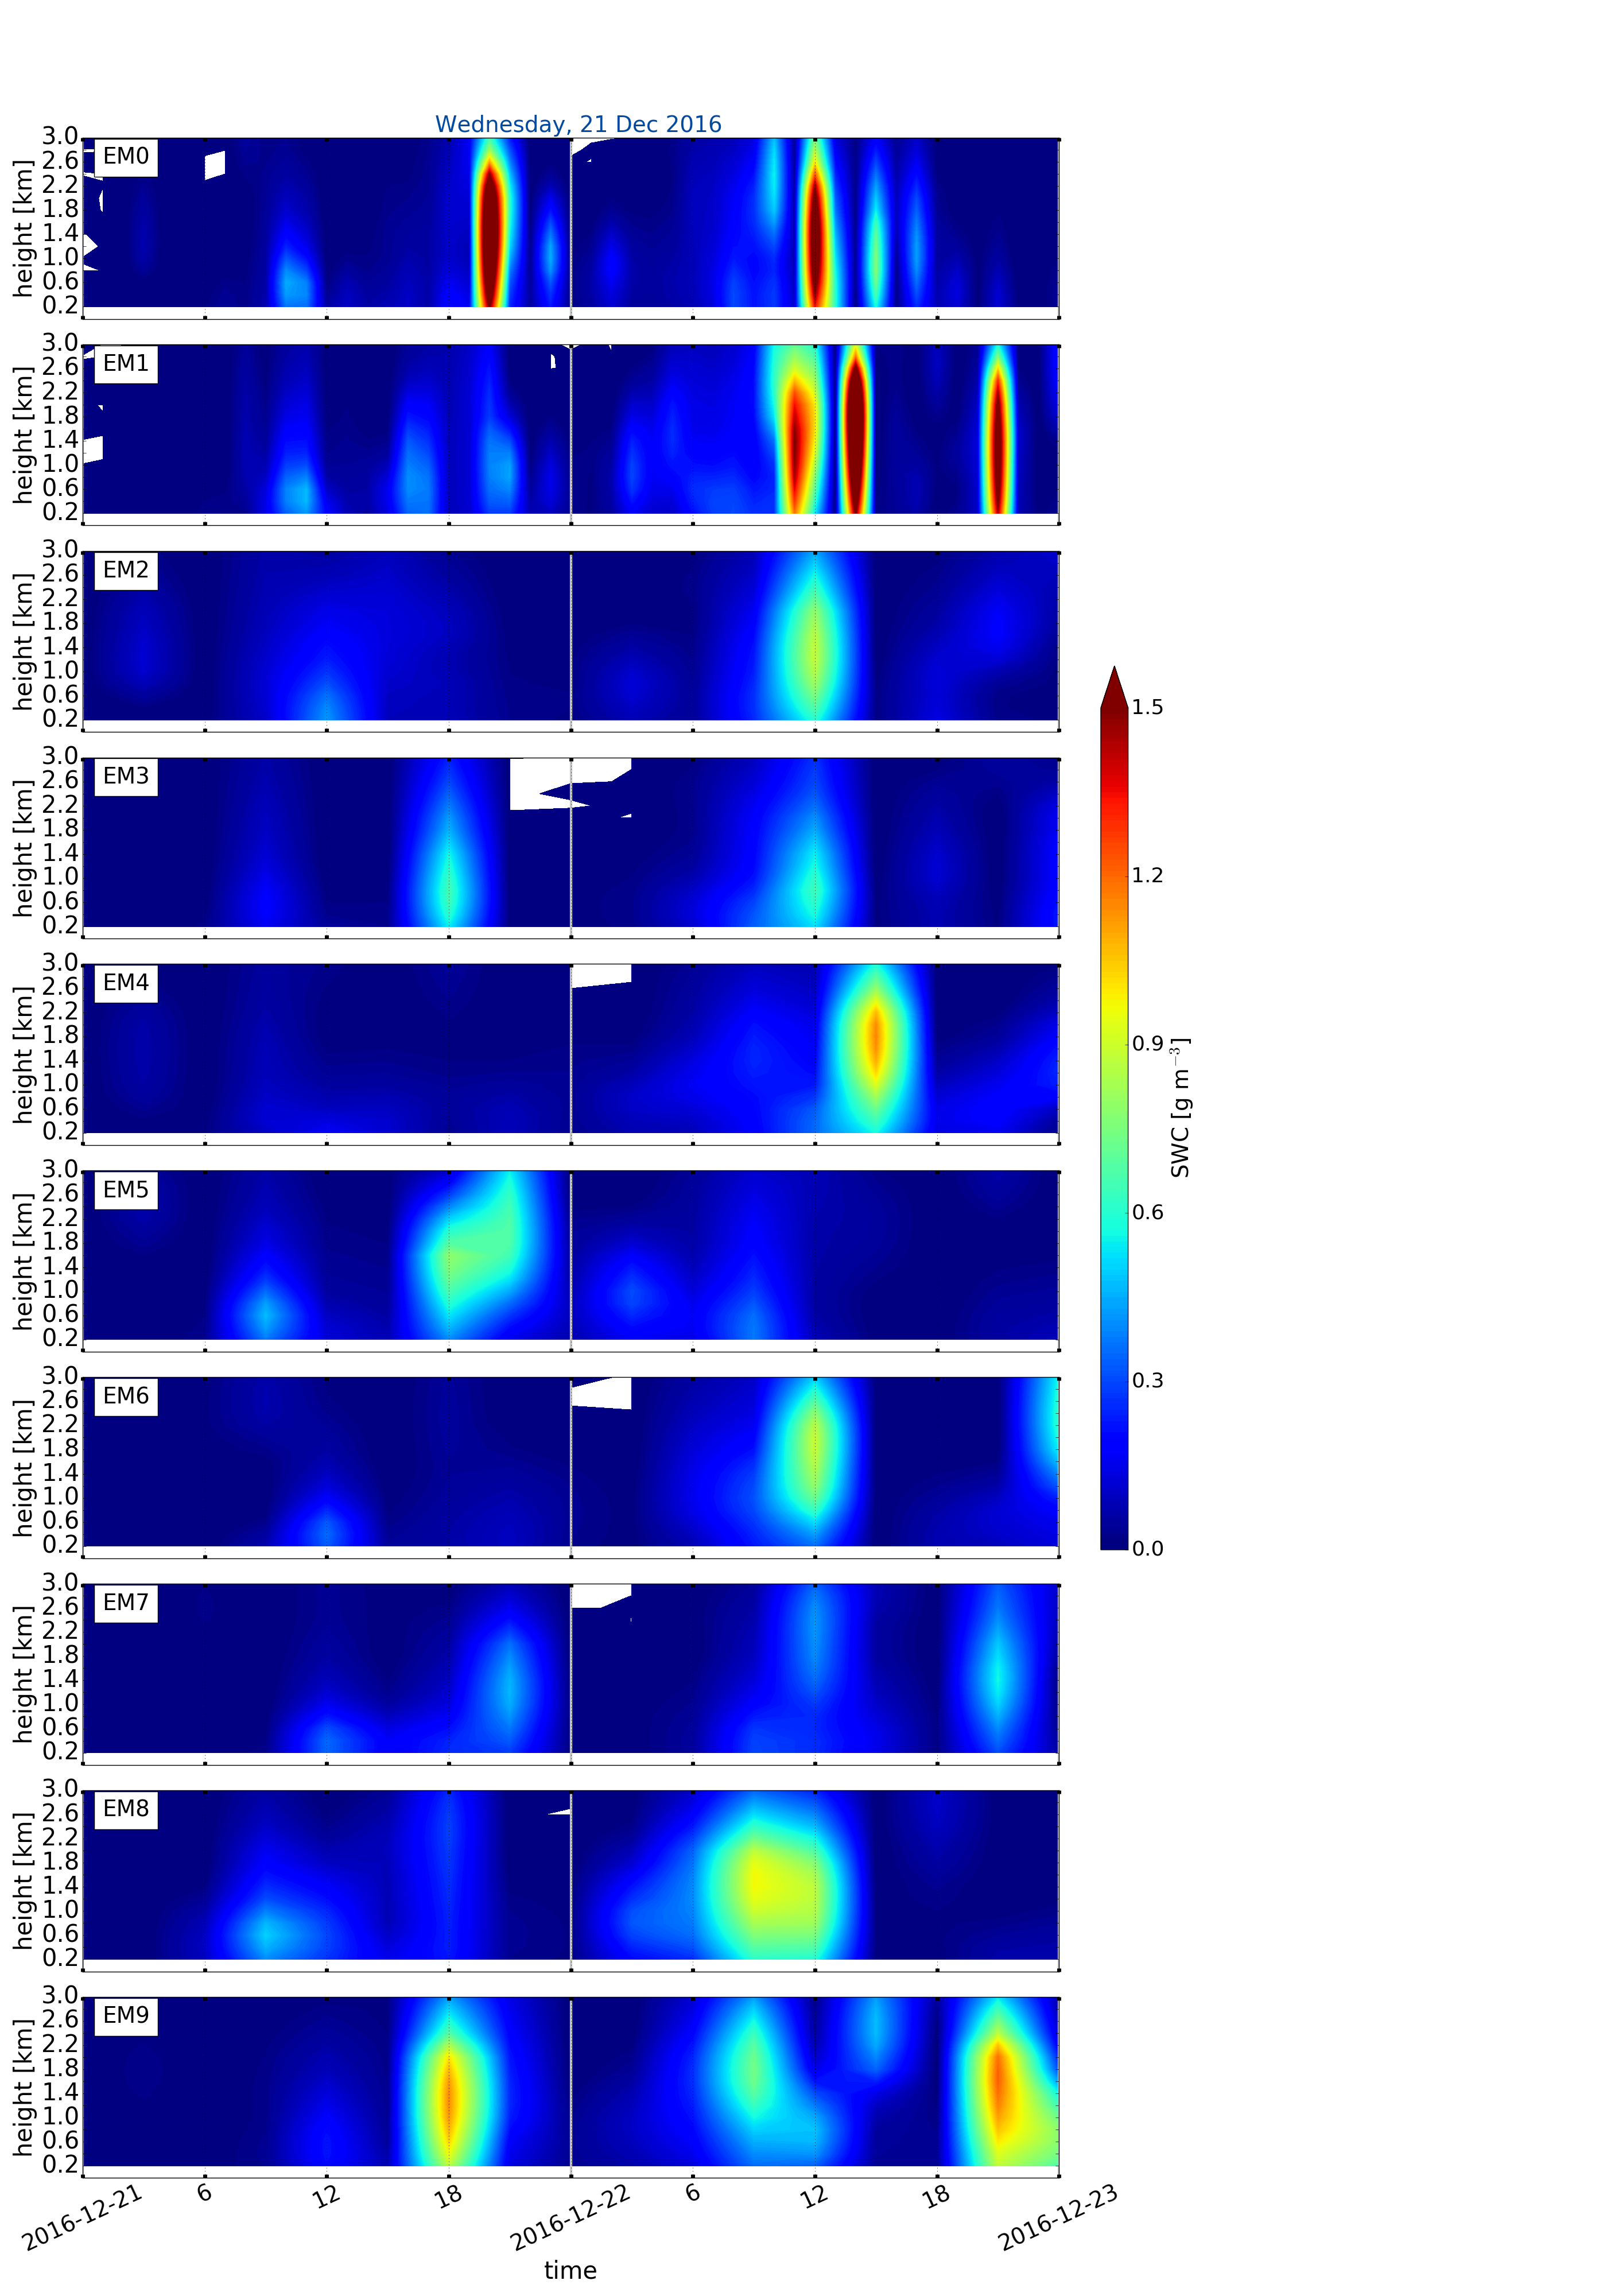
\includegraphics[trim={0cm 0cm 18.3cm 5.1cm},clip,width=0.8\textwidth]{./fig_09EM/20161221}
	\caption{SWC of all ensemble members initialised Wednesday, \SI{21}{\dec} at 0\SI{0}{\UTC} forecast for \SI{48}{\hour}.}\label{fig:EM09_21}
\end{figure}
%%%%%%%%%%%%%%%%%%%%%%%%%%%%%%%%%%%%%%%%%%%%%%%%%%%%%%%%%%%%%%%%%%%%%%%%%%
%
\textcolor{red}{DISCUSSION! Why does MEPS not catch that peak at \SI{16}{\UTC}? Maybe because it is too close to the up-slope storm. Also, Why is the control so high compared to the perturbed members? It catches the up-slope part when also a little weak. Most of the ensemble members would have caught it around \SI{9}{\UTC}. One ensemble member has predicted a high value of SWC at \SI{18}{\UTC}, compare to \Cref{fig:EM09_21}. Why is the up-slope storm more consistent compared to the pulsing? Regional effects? MEPS does well even with catching the pulses and up-slopes, at Haukeliseter is a very difficult orography. }
% %
\newline \noindent
The vertical temperature profile performed with MEPS in \Cref{fig:meps_sound_20} and \ref{fig:meps_sound_21}, shows that an initialisation \SI{36}{\hour} prior to the event would give a cloud with height up to \SI{3}{\km}, as observed in \Cref{fig:SWC21} first panel. An initialisation closer to the occurrence of the storm shows, that MEPS underestimates the intensity and height of the storm (\Cref{fig:meps_sound_21}).
%
%%% image sounding MEPS %%%%%%%%%%%%%%%%%%%%%%%%%%%%%%%%%%%%%
% !TeX spellcheck = en_GB
\begin{figure}
	\centering
	\begin{subfigure}[b]{0.49\textwidth}
		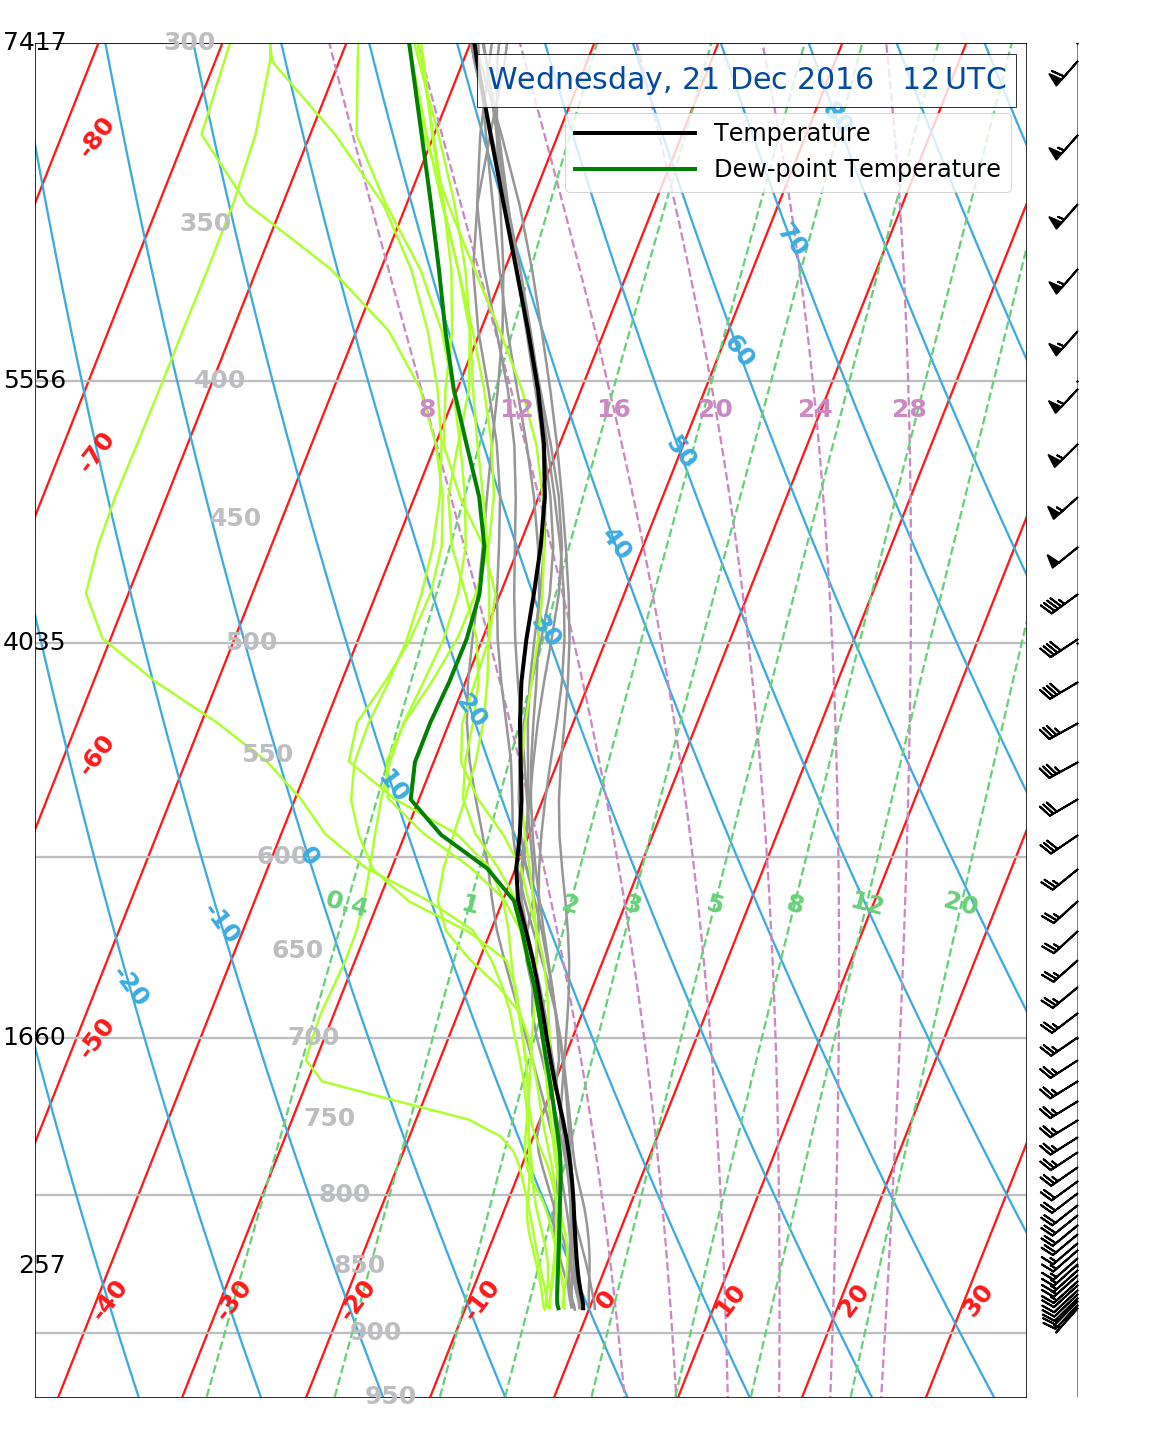
\includegraphics[width=\textwidth]{./fig_Sounding/20161220_36}
		\caption{}\label{fig:meps_sound_20}
	\end{subfigure}
	\begin{subfigure}[b]{0.49\textwidth}
		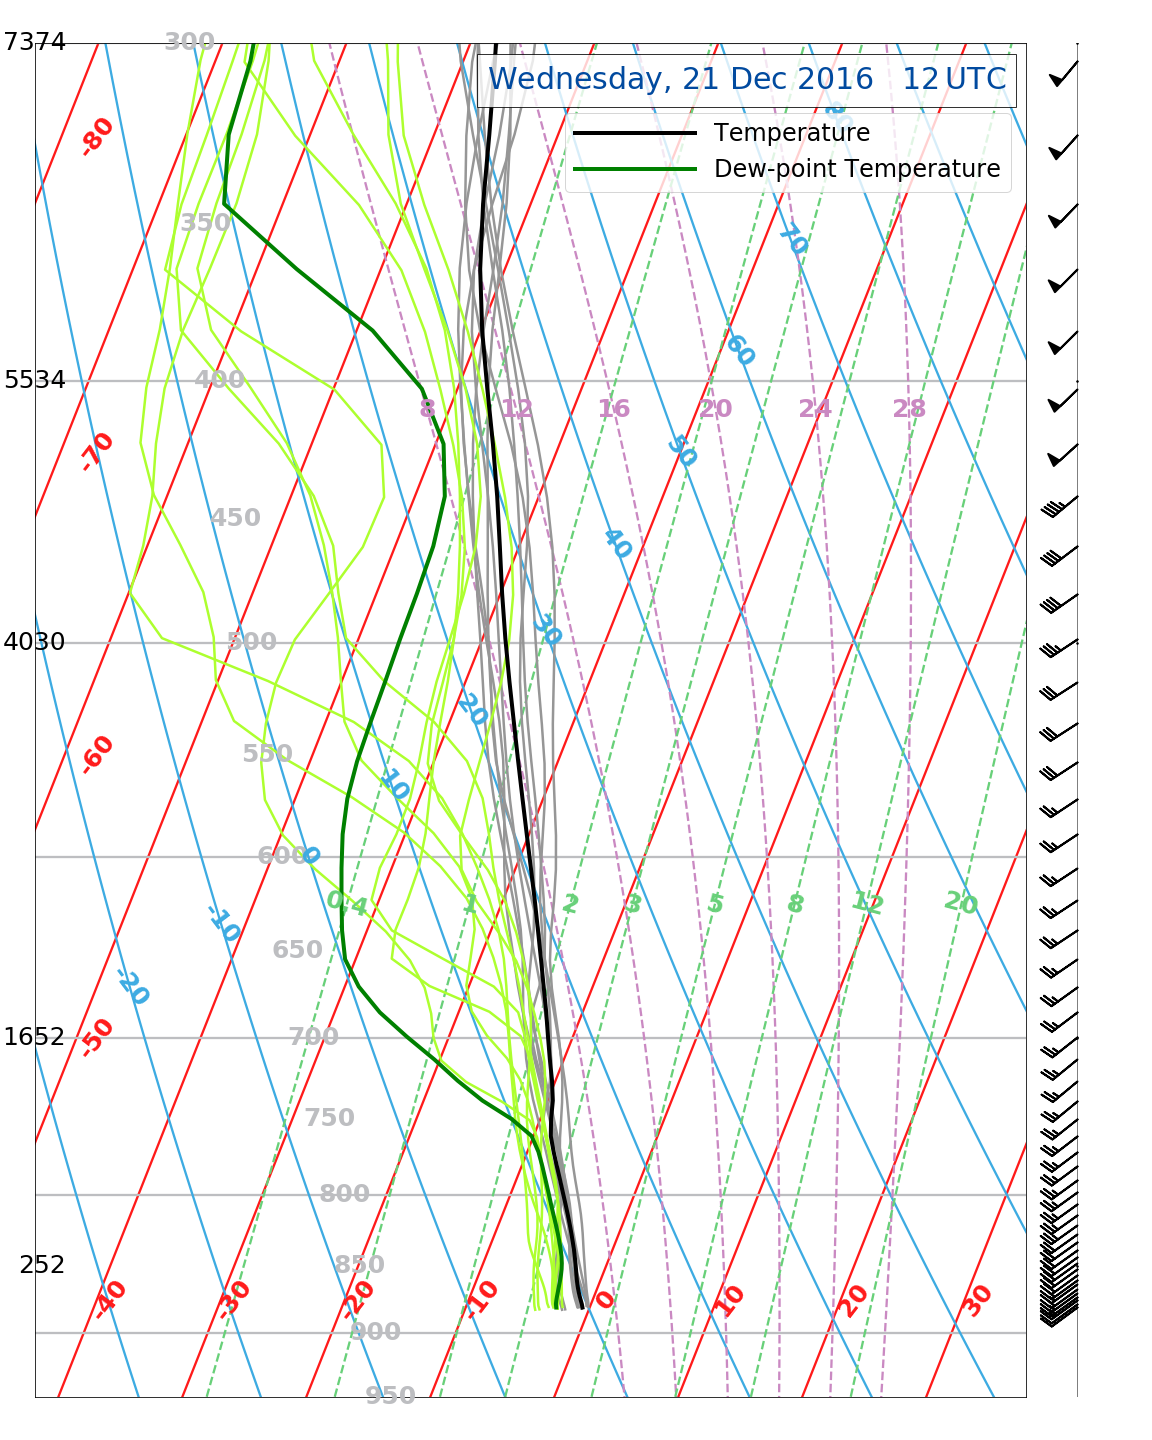
\includegraphics[width=\textwidth]{./fig_Sounding/20161221_12}
		\caption{}\label{fig:meps_sound_21}
	\end{subfigure}
	\caption{Vertical temperature profiles produced with MEPS. \protect{\subref{fig:meps_sound_20}} is initialised: Tuesday, \SI{20}{\dec} \SI{00}{\UTC}. \protect{\subref{fig:meps_sound_21}} is initialised: Wednesday, \SI{21}{\dec} \SI{00}{\UTC}.}
\end{figure}
%%%%%%%%%%%%%%%%%%%%%%%%%%%%%%%%%%%%%%%%%%%%%%%%%%%%%%%%%%%%%%%%%%%%%%%%%%
\textcolor{red}{DISCUSSION! Bring all into relation with the coefficient of variation.}



%%%%%%%%%%%%%%%%%%%%%%%%%%%%%%%%%%%%%%%%%%%%%%%%%%%%%%%%%%%%%%%%%%%%%%%%
\subsection{Saturday, \SI{24}{\dec}}
%%%%%%%%% vertical obs %%%%%%%%%%%%%%
%\subsection{Vertical snowfall observations}
\label{sec:vertEM09:2412}
% %%% image SWP %%%%%%%%%%%%%%%%%%%%%%%%%%%%%%%%%%%%%
\begin{figure}[t]
	\centering
	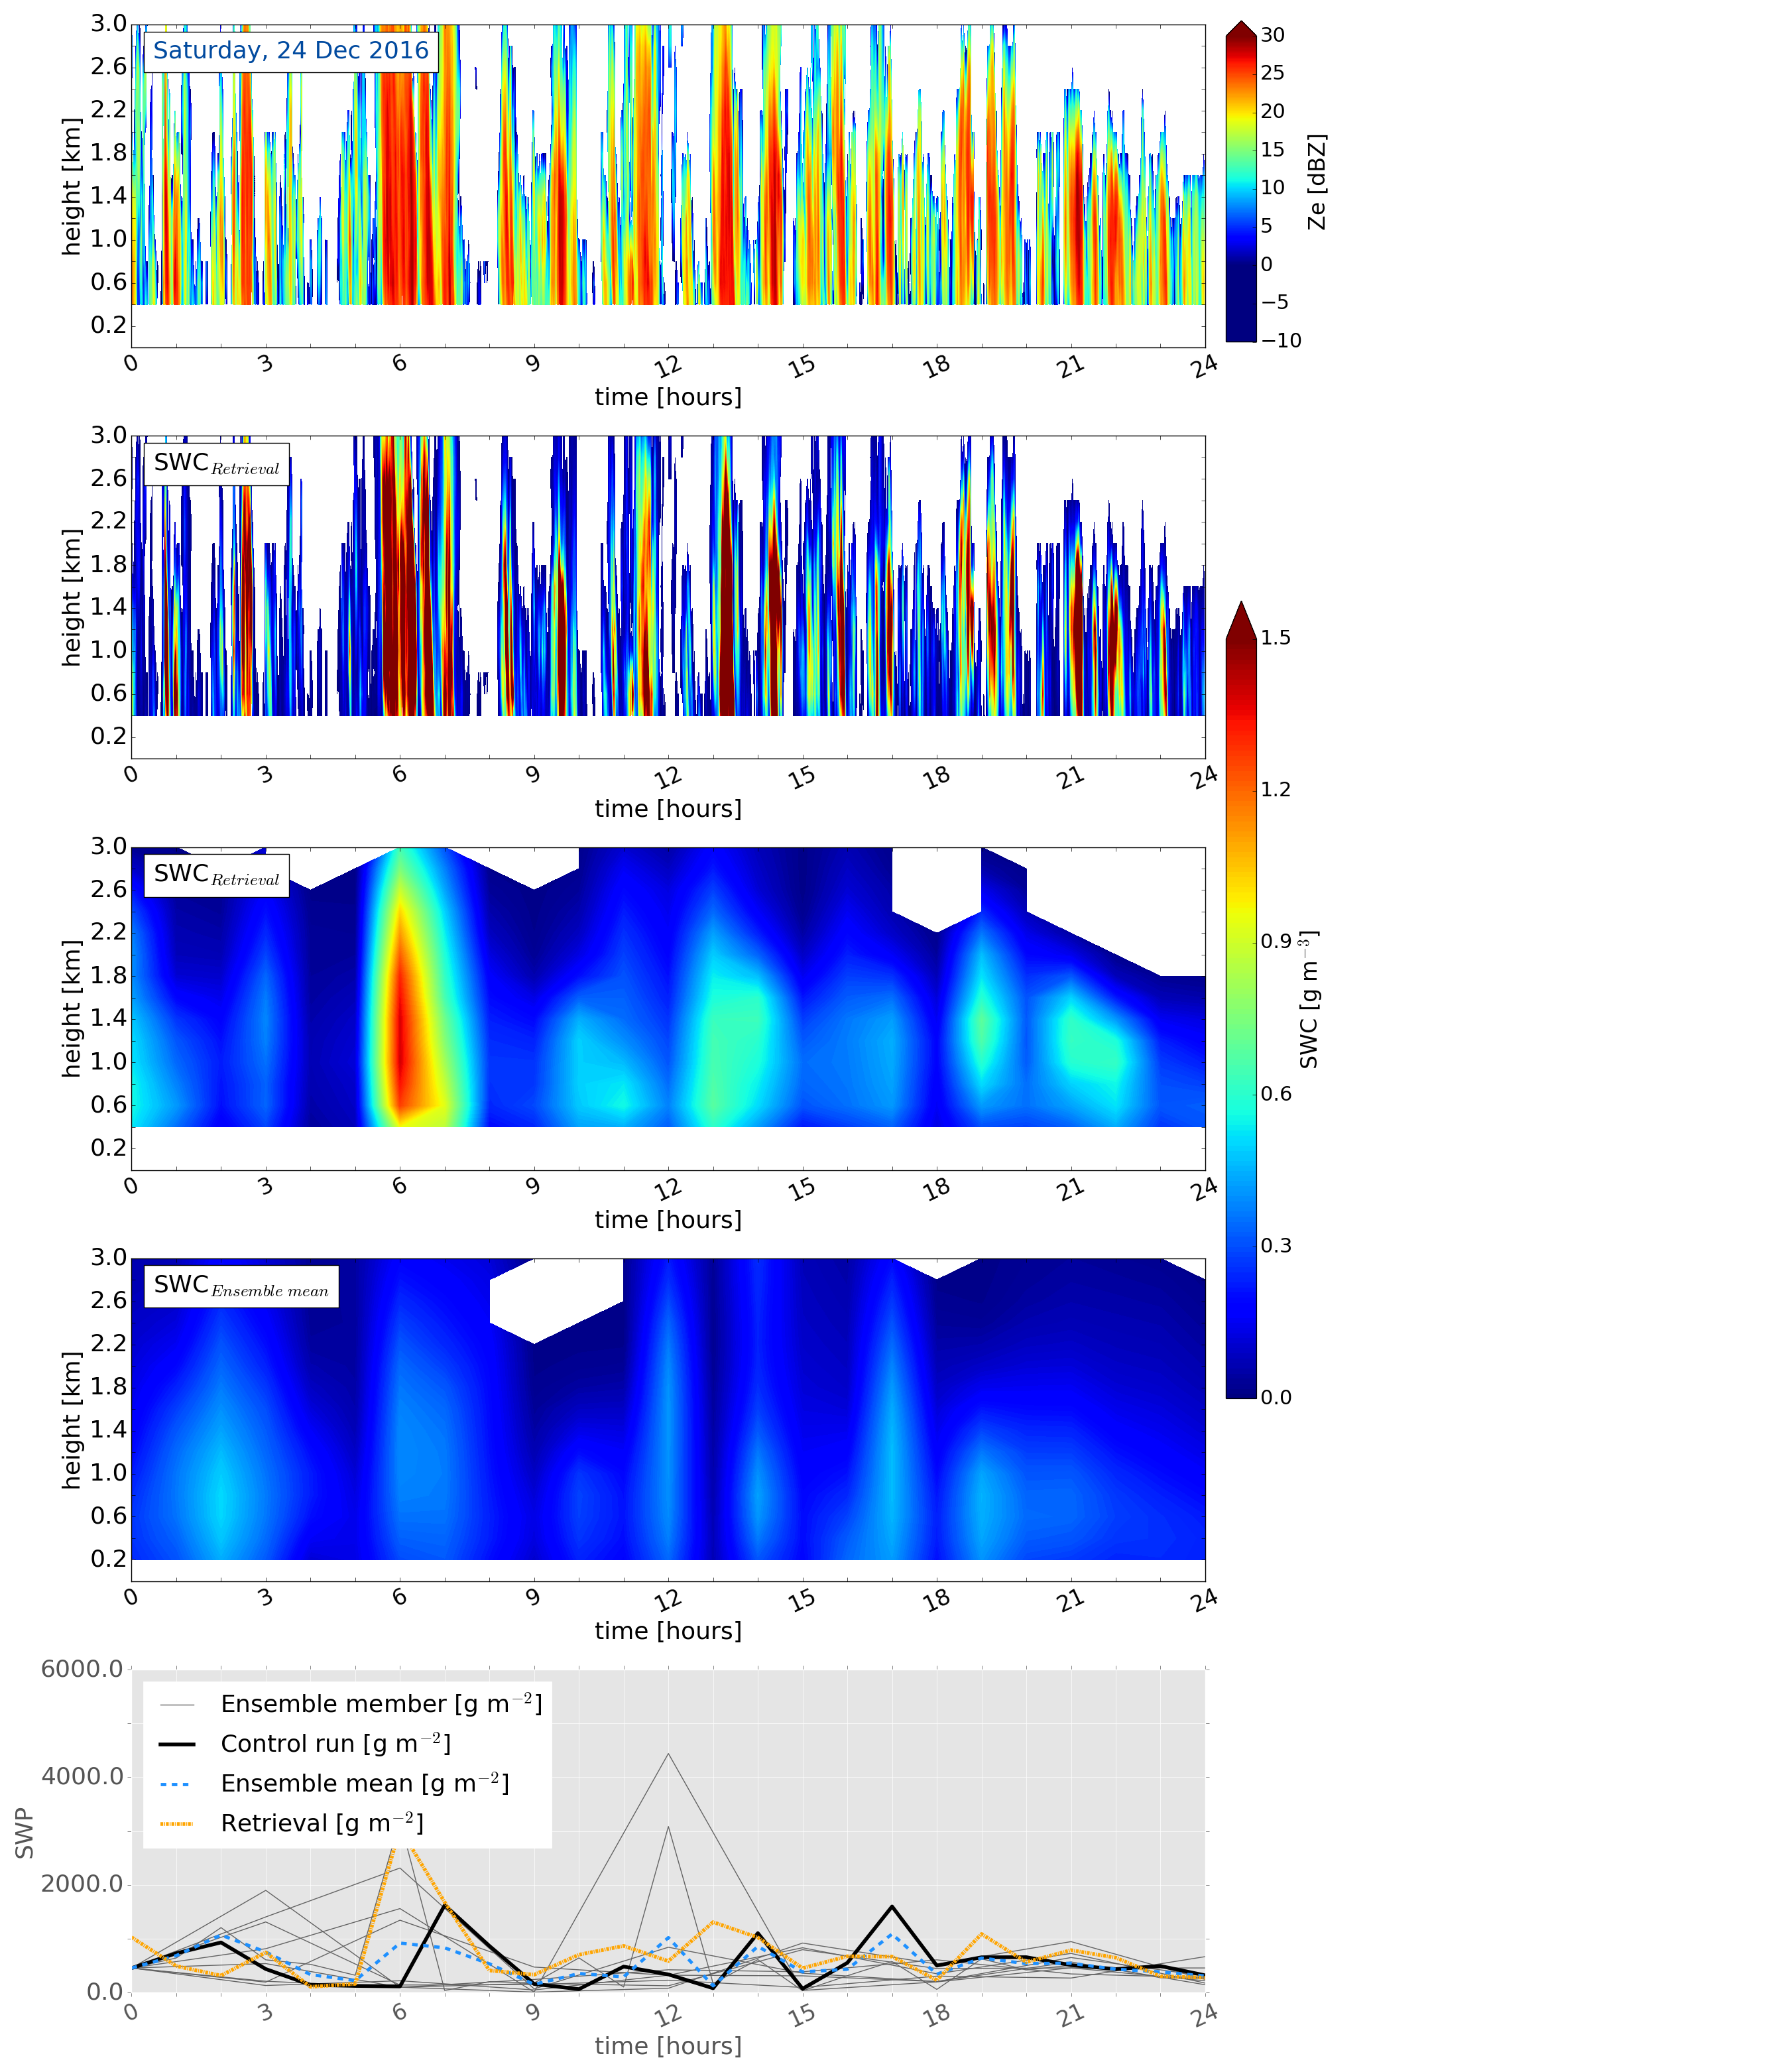
\includegraphics[trim={0.4cm .4cm 31.3cm 63.5cm},clip,width=\textwidth]{./fig_SWC/20161224}
	\caption{}\label{fig:SWP24}
\end{figure}
%%%%%%%%%%%%%%%%%%%%%%%%%%%%%%%%%%%%%%%%%%%%%%%%%%%%%%%%%%%%%%%%%%%%%%%%%%
% text
%
% %%% image ensemble member 0-9 %%%%%%%%%%%%%%%%%%%%%%%%%%%%%%%%%%%%%
\begin{figure}[t]
	\centering
	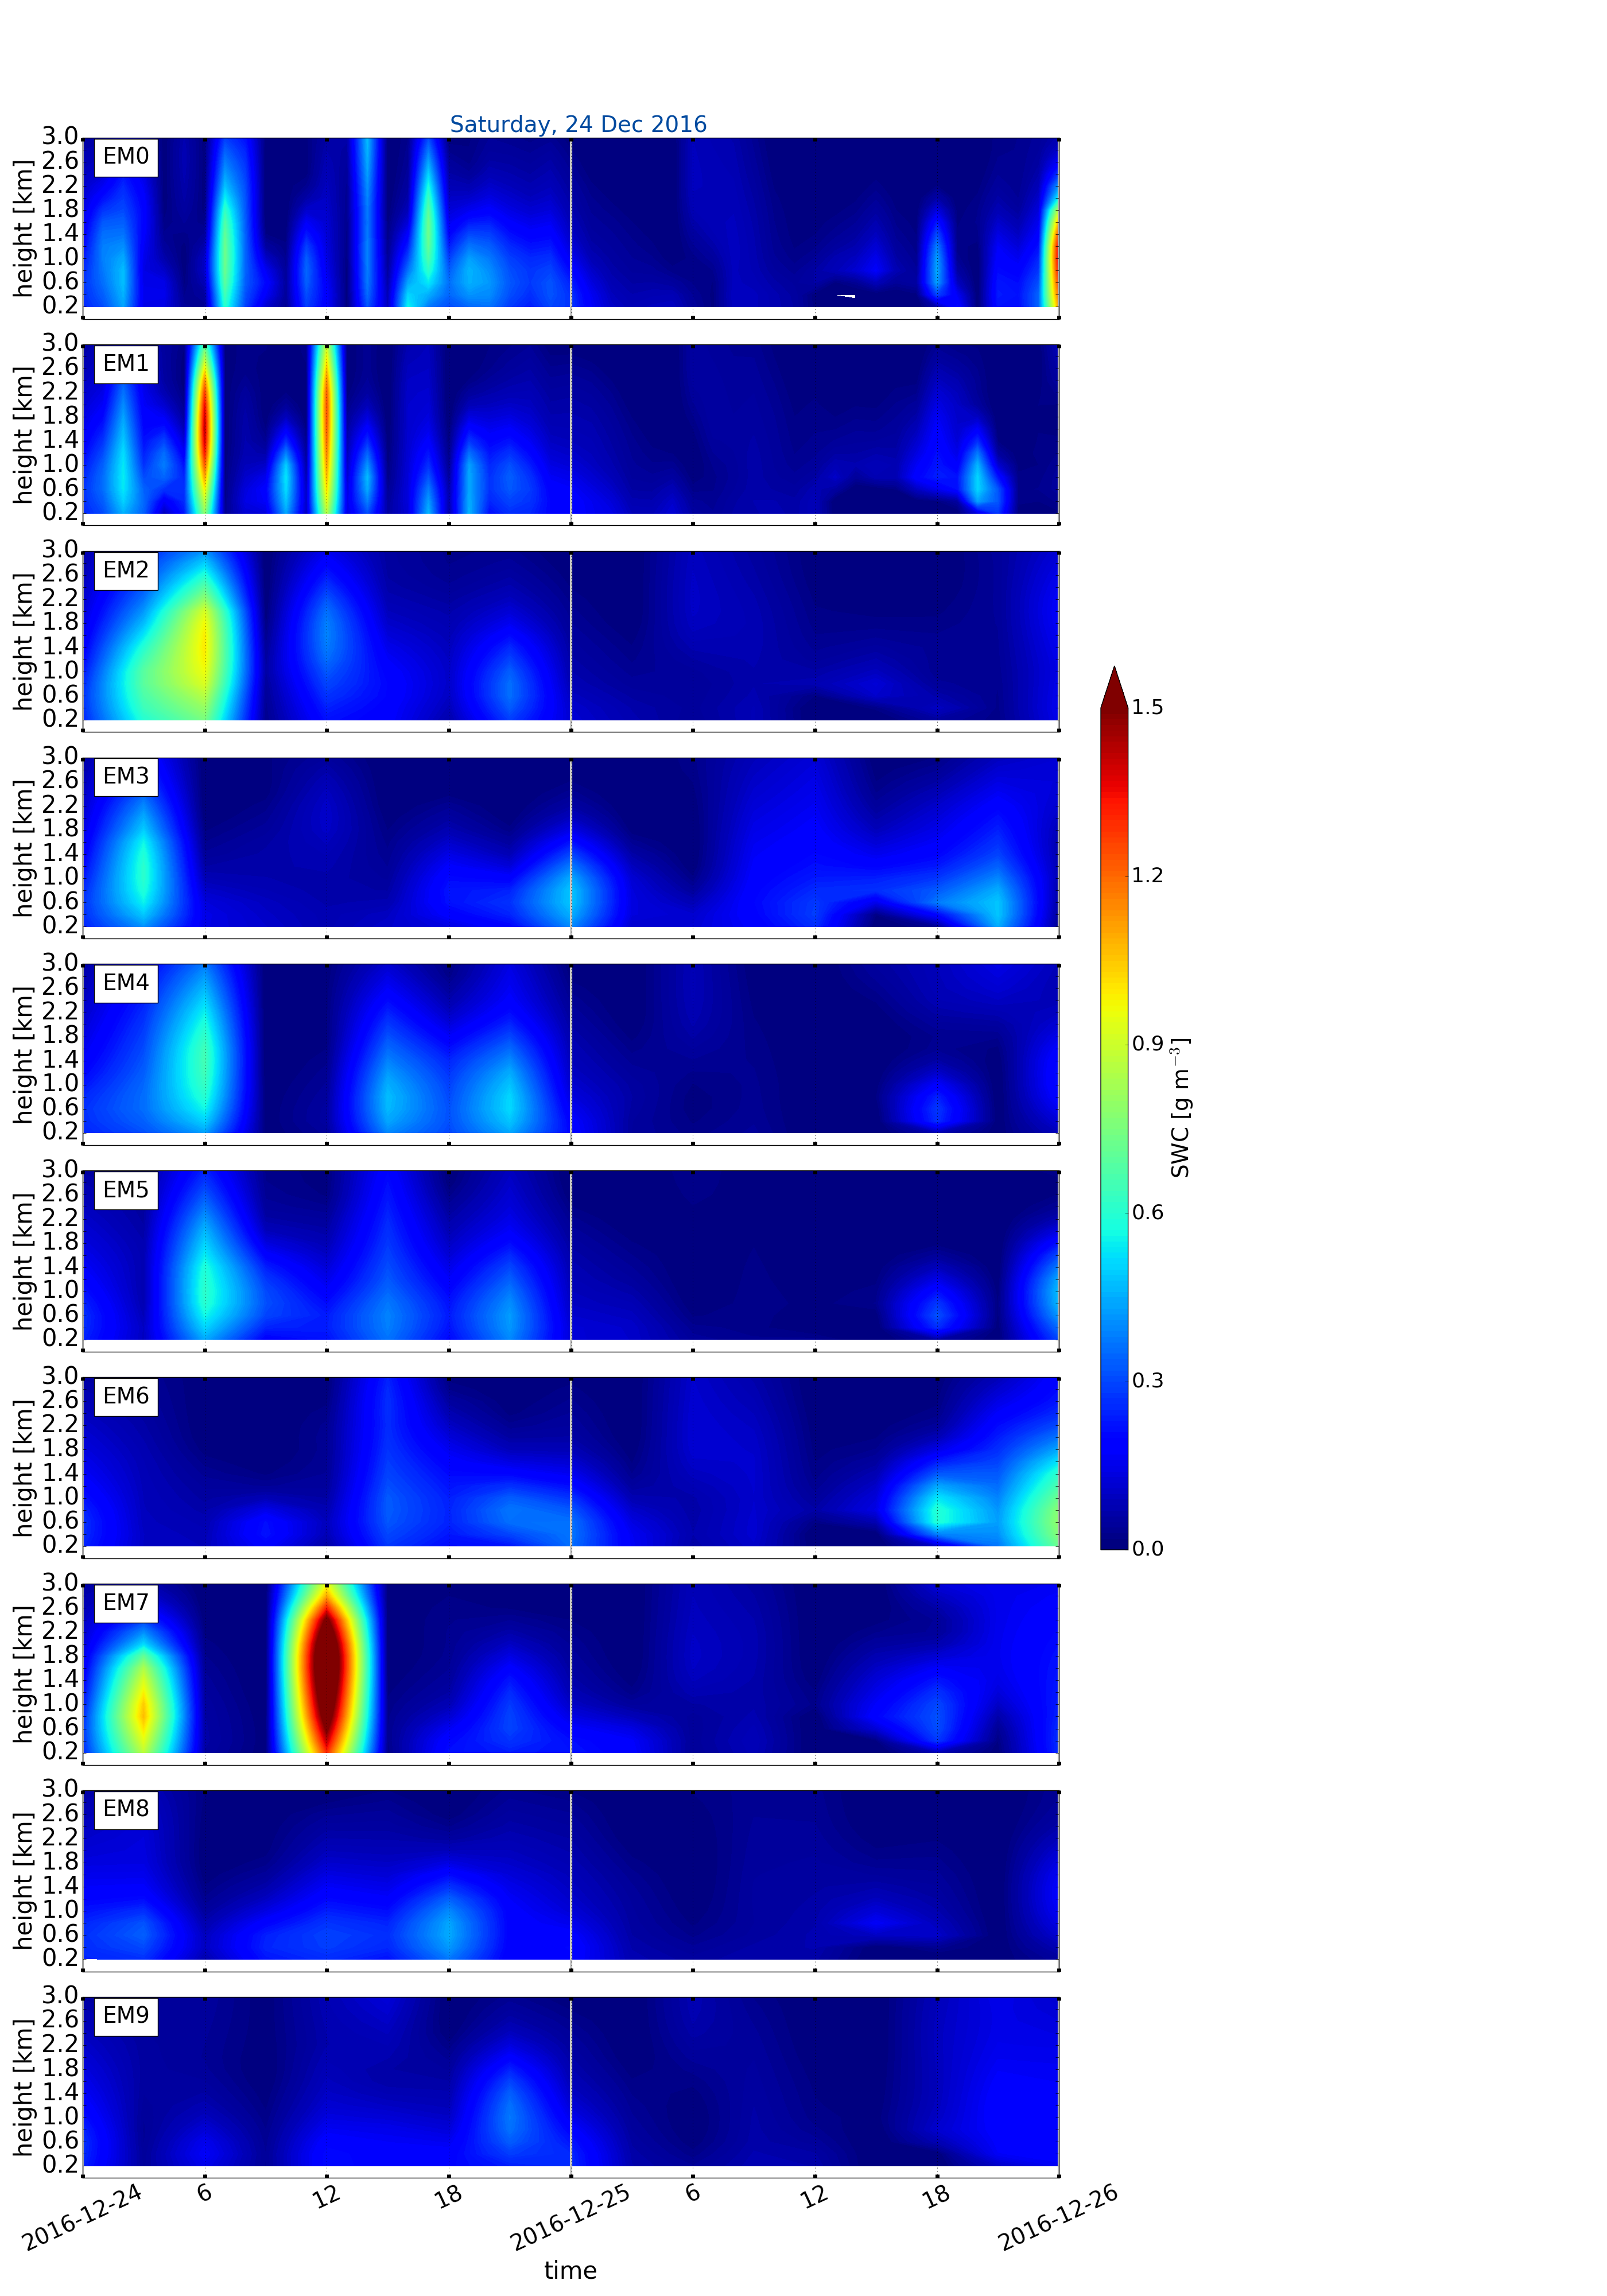
\includegraphics[trim={0cm 0cm 18.3cm 5.1cm},clip,width=0.8\textwidth]{./fig_09EM/20161224}
	\caption{SWC of all ensemble members initialised Saturday, \SI{24}{\dec} at 0\SI{0}{\UTC} forecast for \SI{48}{\hour}.}\label{fig:EM09_24}
\end{figure}
%%%%%%%%%%%%%%%%%%%%%%%%%%%%%%%%%%%%%%%%%%%%%%%%%%%%%%%%%%%%%%%%%%%%%%%%%%
\textcolor{red}{DISCUSSION! Bring all into relation and include the verification plots}
\begin{itemize}
	\item Because EM3, EM4, EM7 to EM9 are only valid every three hours can precipitation peaks not crop up in such a high frequency as for example the deterministic forecast. 
\end{itemize}


%%%%%%%%%%%%%%%%%%%%%%%%%%%%%%%%%%%%%%%%%%%%%%%%%%%%%%%%%%%%%%%%%%%%%%%%
\subsection{Sunday, \SI{25}{\dec}}
%%%%%%%%% vertical obs %%%%%%%%%%%%%%
%\subsection{Vertical snowfall observations}
\label{sec:vertEM09:2512}
% %%% image SWP %%%%%%%%%%%%%%%%%%%%%%%%%%%%%%%%%%%%%
\begin{figure}[t]
	\centering
	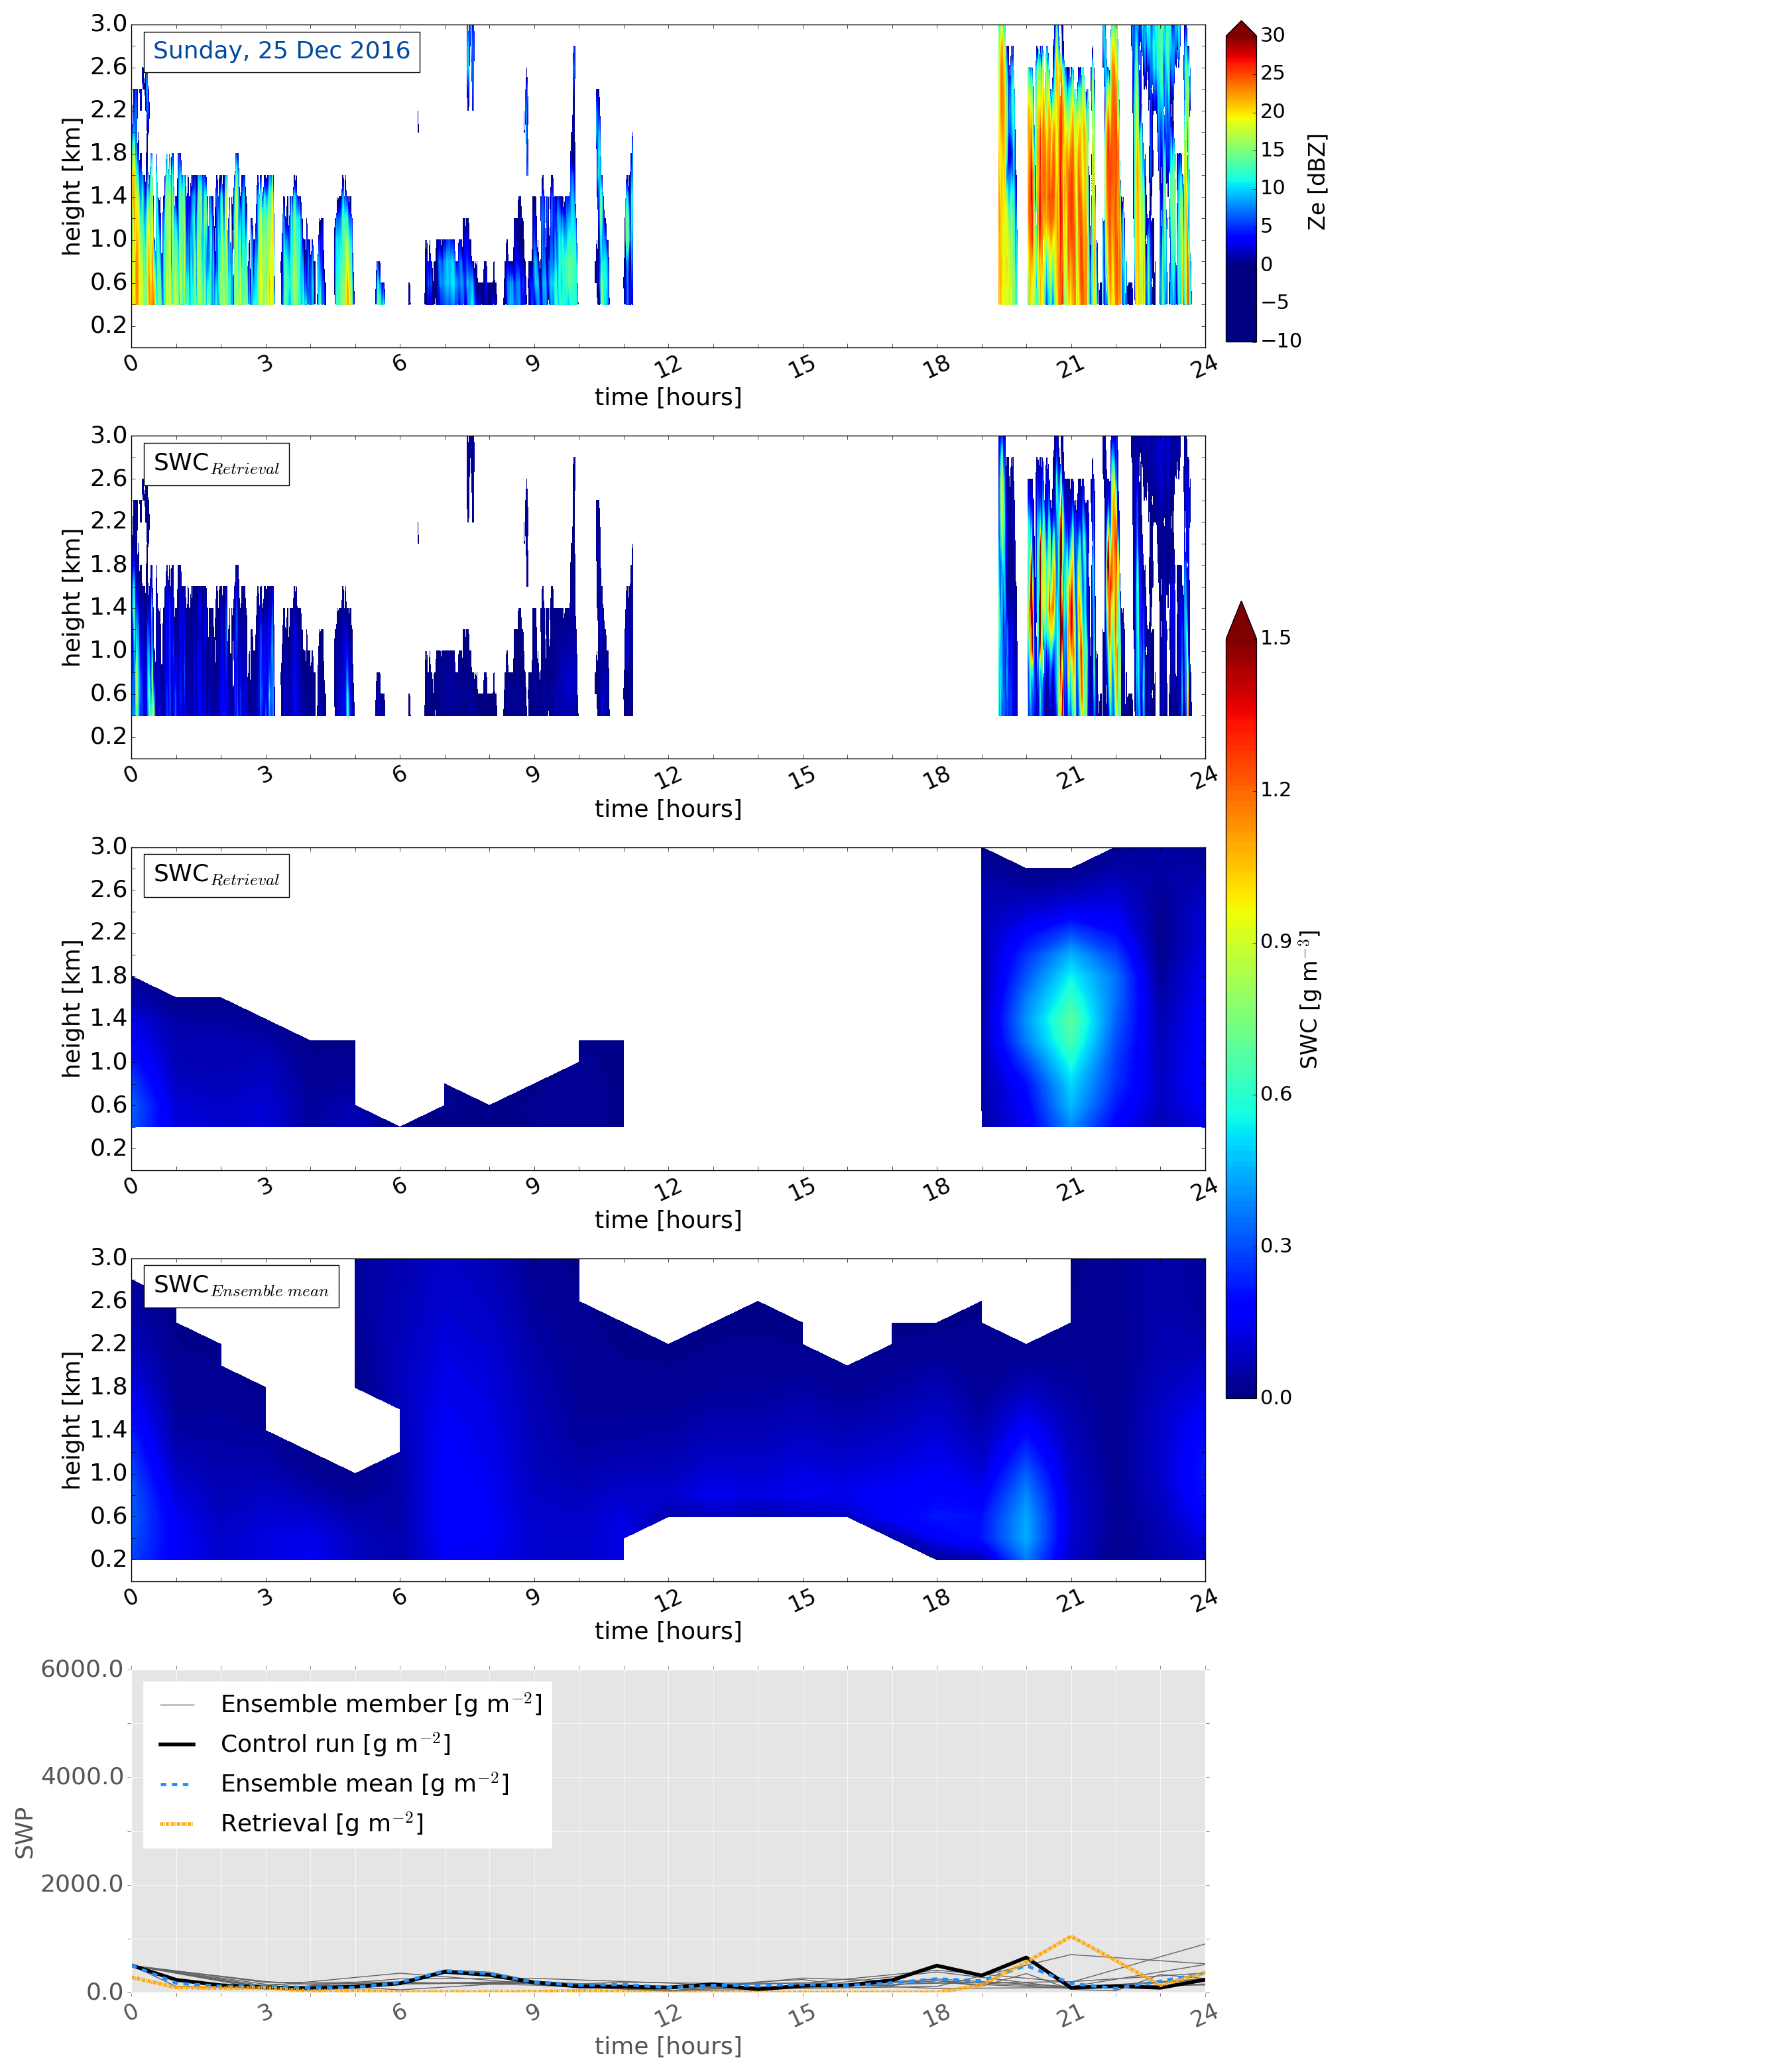
\includegraphics[trim={0.4cm .4cm 31.3cm 63.5cm},clip,width=\textwidth]{./fig_SWC/20161225}
	\caption{}\label{fig:SWP25}
\end{figure}
%%%%%%%%%%%%%%%%%%%%%%%%%%%%%%%%%%%%%%%%%%%%%%%%%%%%%%%%%%%%%%%%%%%%%%%%%%
% text
%
% %%% image ensemble member 0-9 %%%%%%%%%%%%%%%%%%%%%%%%%%%%%%%%%%%%%
\begin{figure}[t]
	\centering
	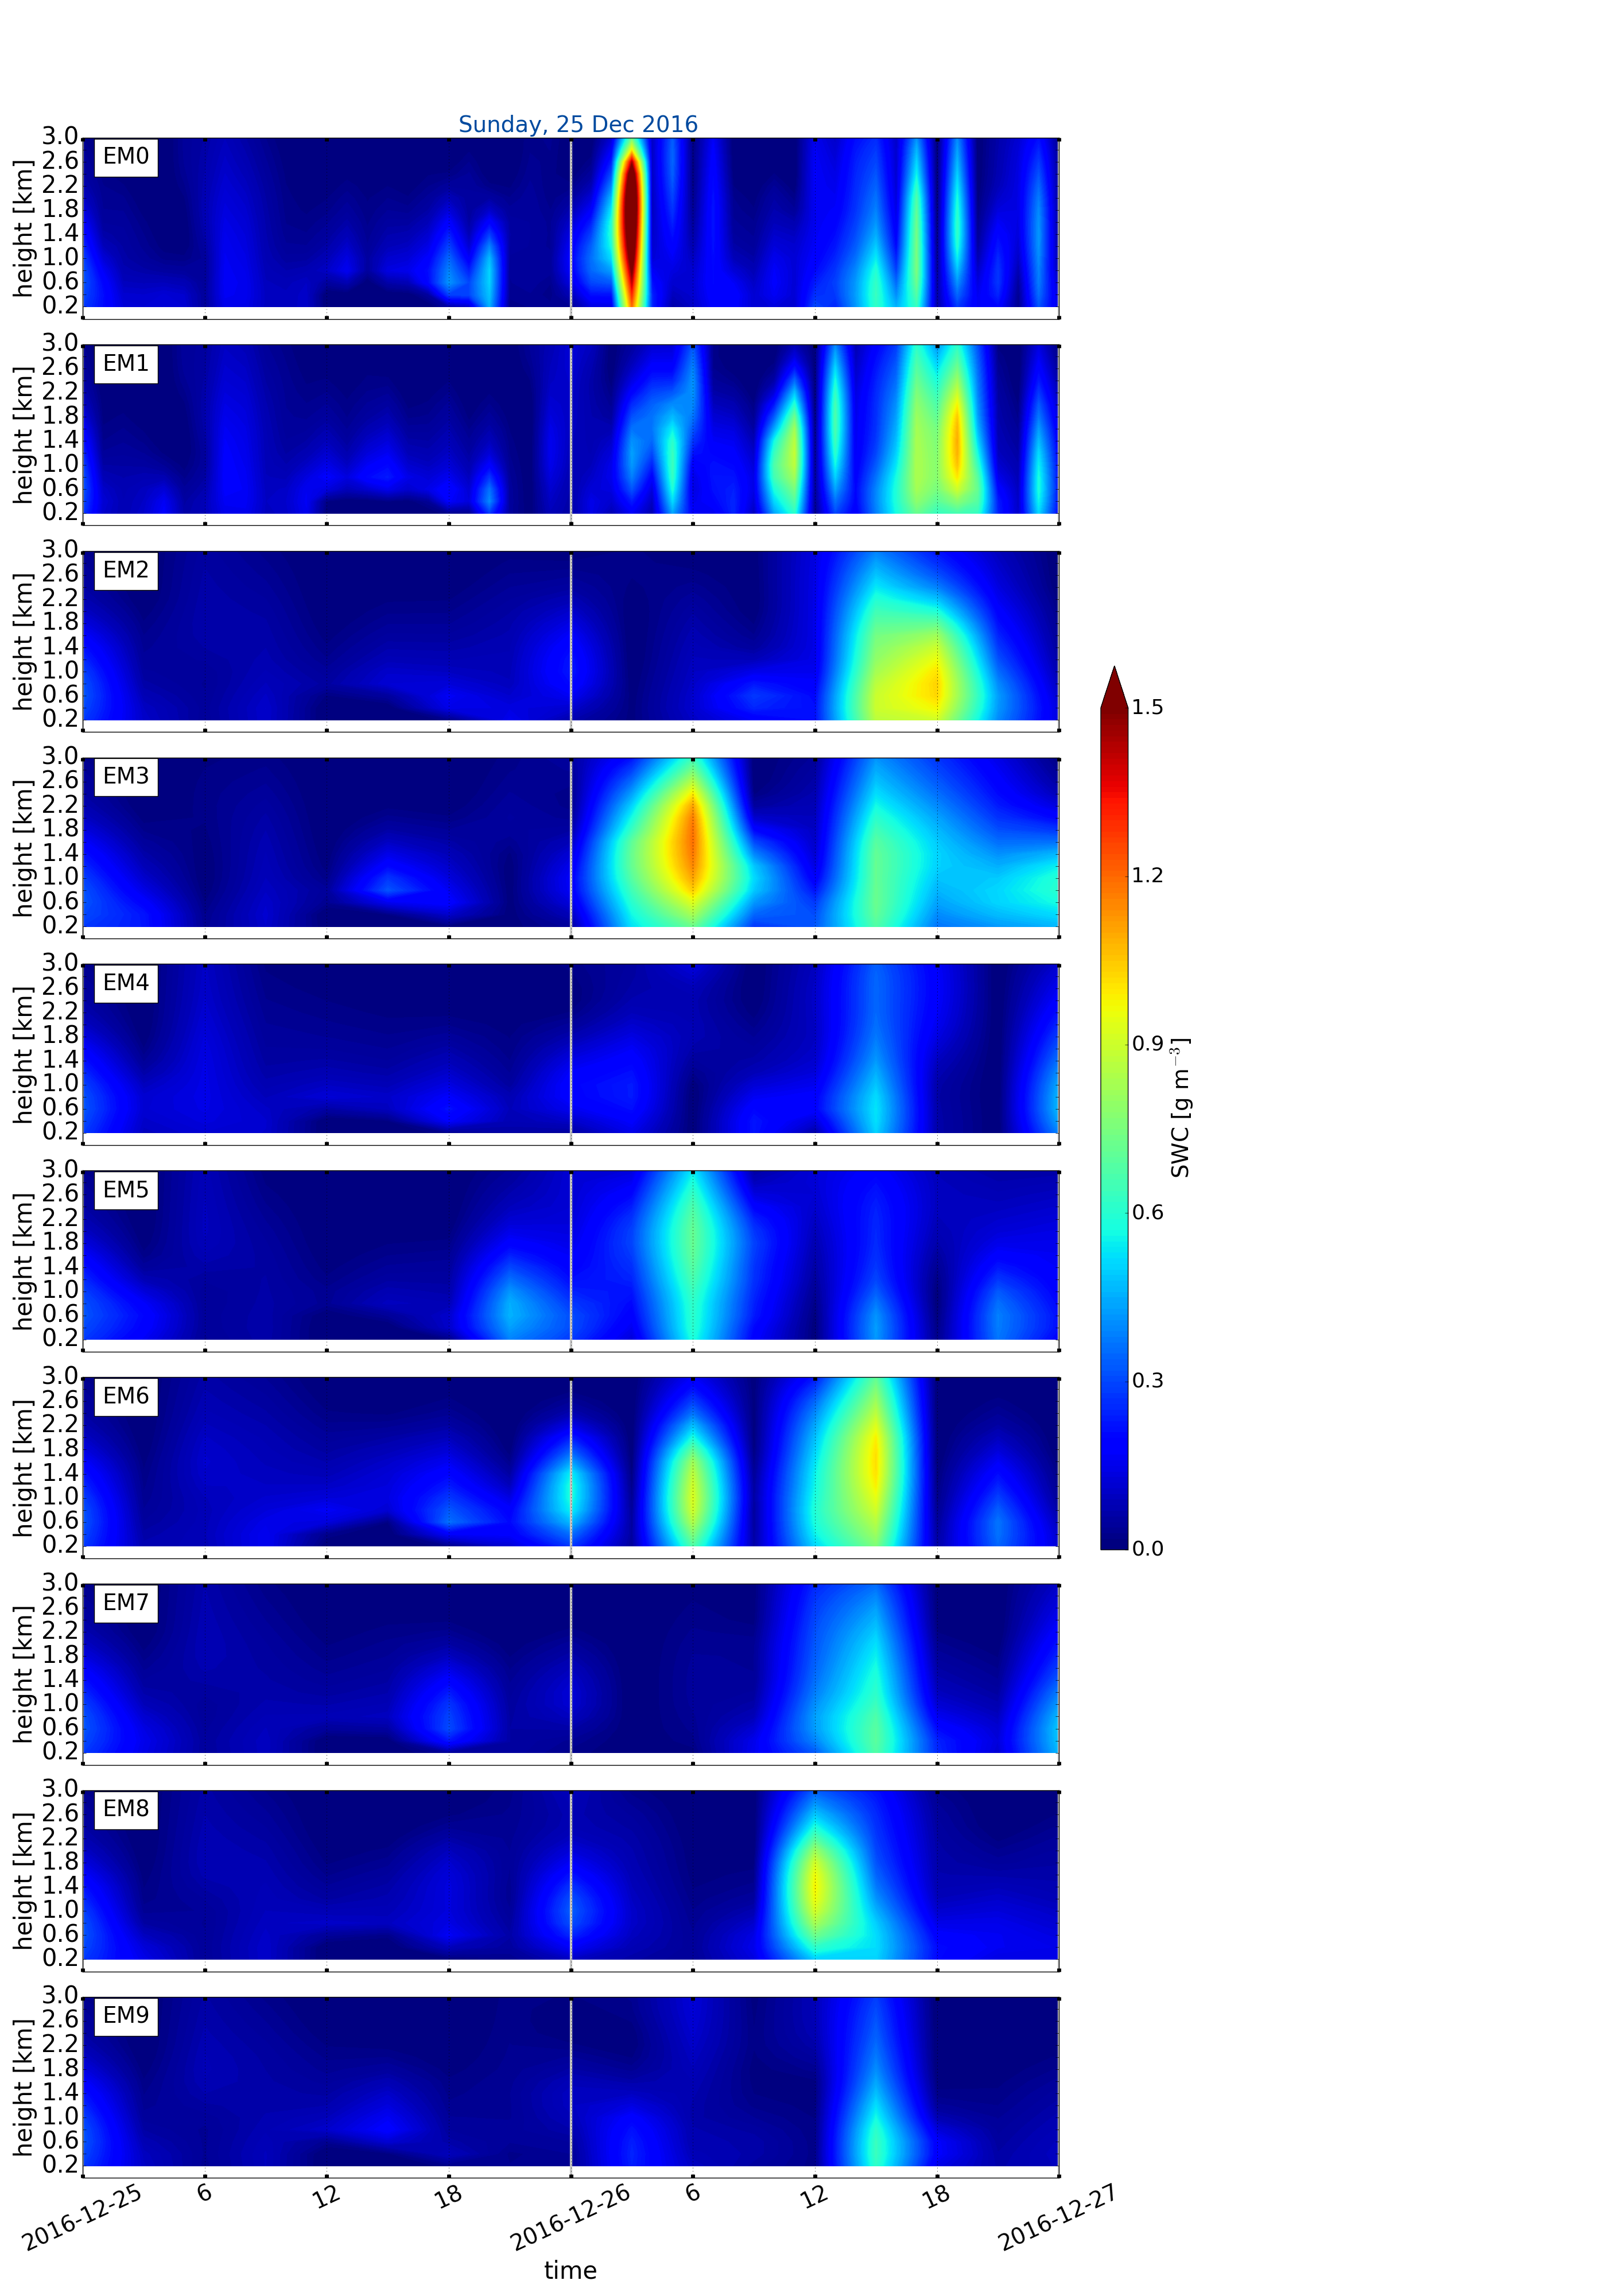
\includegraphics[trim={0cm 0cm 18.3cm 5.1cm},clip,width=0.8\textwidth]{./fig_09EM/20161225}
	\caption{SWC of all ensemble members initialised Sunday, \SI{25}{\dec} at 0\SI{0}{\UTC} forecast for \SI{48}{\hour}.}\label{fig:EM09_25}
\end{figure}
%%%%%%%%%%%%%%%%%%%%%%%%%%%%%%%%%%%%%%%%%%%%%%%%%%%%%%%%%%%%%%%%%%%%%%%%%%
\textcolor{red}{DISCUSSION! Bring all into relation and include the verification plots}
%%%%%%%%%%%%%%%%%%%%%%%%%%%%%%%%%%%%%%%%%%%%%%%%%%%%%%%%%%%%%%%%%%%%%%%%